\documentclass{article}
\usepackage{iclr2027_conference,times}
\input{math_commands.tex}
\usepackage{amsmath,amssymb,amsthm,booktabs,graphicx,enumitem,xcolor}
\usepackage{hyperref}
\usepackage{url}
\usepackage{microtype}
\newtheorem{proposition}{Proposition}
\newtheorem{theorem}{Theorem}
\newtheorem{lemma}{Lemma}
\newtheorem{corollary}{Corollary}
\newtheorem{remark}{Remark}
\newcommand{\fhat}{\hat{f}}
\newcommand{\code}[1]{\texttt{\small #1}}

\title{From Residual Identification to Task Repair in Frozen Vision--Language--Action Policies}
\author{Anonymous authors}
\begin{document}
\maketitle

\begin{abstract}
A robot can identify a disturbance accurately and still fail to compensate for it.
We study this gap at the action interface of frozen vision--language--action policies,
where a healthy motion model and calibrated residuals drive bounded online corrections.
We analyze residual information, correction authority and closed-loop stability as separate
links between disturbance estimation and task repair.
This decomposition yields exact local cancellation conditions, a physical-error bound under
calibration mismatch, and a conditional stability analysis for composite position feedback.
Constructed examples show why accurate inversion, a smaller fitted objective, or stable
healthy dynamics can each be insufficient.
Experiments include historical command-offset results on four LIBERO suites, 2,220 new
all-joint physical-fault confirmation rollouts on Panda and ALOHA, and a separate 5,424-rollout
estimator tuning study. Weighted allocation improves the prespecified Panda joint-5 comparison
from 15/60 to 41/60, but harms another condition. Composite adaptation does not establish an
advantage over Kalman on independent ALOHA confirmation. The resulting framework connects
observer design to correction authority and task evidence, while exposing the remaining
gap between better tracking and reliable manipulation.
\end{abstract}

\section{Introduction}
\label{sec:introduction}
Vision--language--action (VLA) policies convert visual and language observations into robot
commands \citep{pi0,pi05,openvla,groot}. Their deployment depends on a second map: how those
commands produce physical motion. An actuator change can alter this map while the policy
and task remain fixed. Comparing measured motion with a healthy prediction offers a direct
way to adapt without retraining the VLA. The central question is whether the discrepancy
identified through this comparison can be turned into a useful correction.

The answer depends on more than observer accuracy. In our historical experiments, a
calibrated adapter substantially repairs command offsets, yet the same architecture reduces
success under a Panda joint-5 torque fault from $12/20$ to $3/20$ with continuous,
translation-only correction (Figure~\ref{fig:interface}). These are different fault protocols,
not conflicting estimates of one treatment effect. They expose the question studied here:
\emph{when does identifying a disturbance actually repair a task?}

\begin{figure}[t]
\centering
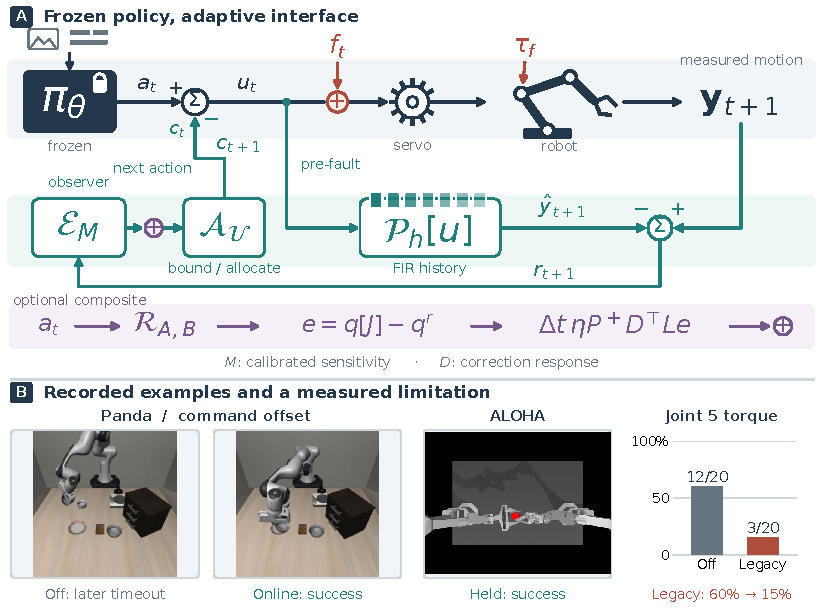
\includegraphics[width=\linewidth]{fig_interface.pdf}
\caption{\textbf{Calibrated interface adaptation and contrasting outcomes.}
The frozen policy emits $a_t$; the adapter sends $u_t=a_t-c_t$. The healthy FIR $\mathcal P_h$
uses known pre-fault commands; estimator $\mathcal E_M$ and bounded rule
$\mathcal A_{\mathcal U}$ update the next correction. Matching purple $\oplus$ ports add
position feedback from reference $\mathcal R_{A,B}$ before projection. Command and torque
faults enter at different levels. Bottom: selected Panda off/online frames, an ALOHA
held-correction success, and measured historical Panda joint-5 success rates with continuous
translation-only correction. Videos illustrate behavior; the chart reports stored outcomes
under a different protocol. Frame provenance and protocols are in Appendix~\ref{app:videos}.}
\label{fig:interface}
\end{figure}

We distinguish \emph{residual information}, \emph{correction authority} and
\emph{closed-loop stability}. The first determines which disturbance effects can be inferred;
the second determines which can be canceled through the permitted inputs; the third concerns
the feedback created by applying an evolving estimate. These requirements can fail
independently. A translation interface may lack a needed motion direction, a fitted inverse
may amplify calibration error, and tracking feedback may destabilize an otherwise stable
observer. Successful contact-rich manipulation requires an additional connection from
controlled state error to the complete task trajectory.

This decomposition organizes both a calibrated adapter and its evaluation. A healthy
finite-impulse-response (FIR) model produces residuals, an observer estimates the disturbance,
and a bounded allocator selects a feasible correction. A composite variant additionally
tracks a healthy position reference driven by raw policy commands. Classical observers and
composite adaptation supply these components; our contribution is to connect their use at
a frozen VLA interface to explicit cancellation conditions and controlled task evidence.

Our contributions are:
\begin{enumerate}[leftmargin=1.5em,itemsep=1pt]
\item \textbf{Cancellation conditions:} exact local criteria and a bound
  relating nominal allocation to physical improvement (Section~\ref{sec:analysis}).
\item \textbf{Feedback analysis:} a common adapter formulation, conditional composite
  stability bounds and exact failure examples (Sections~\ref{sec:framework}--\ref{sec:analysis}).
\item \textbf{Tests across joints and tasks:} independent confirmations on every Panda and ALOHA arm
  joint, three LIBERO suites and six tuned observer families (Section~\ref{sec:evaluation}).
\end{enumerate}

\section{Related work}
\label{sec:related}
\textbf{Where adaptation enters the robot stack.} Generalist policies learn the mapping
from observations to actions through token prediction \citep{rt2,openvla}, diffusion
\citep{diffusionpolicy,octo}, or flow-based action generation \citep{pi0,pi05}.
OFT studies efficient VLA fine-tuning and action representations \citep{openvlaoft}.
These approaches improve the policy; the present problem is a deployment change in the
map from its actions to motion. Keeping that distinction explicit separates action-interface
adaptation from representation transfer, policy fine-tuning and task learning.

\textbf{What is learned and what is corrected.} Adaptive augmentation of a pretrained policy
is established: \citet{cheng2022l1rl} combine reinforcement learning with $\mathcal L_1$
adaptive control, and DATT combines a learned trajectory controller with an $\mathcal L_1$
disturbance estimator \citep{huang2023datt}. Residual policy learning trains an additive action
\citep{silver2018residual,johannink2019residual}; RMA trains a policy to consume an adapted
context \citep{kumar2021rma}. Our adapter instead estimates a disturbance from calibrated
proprioceptive residuals. This choice leaves the VLA frozen but requires checking that its
available correction coordinates can influence the affected motion. The surrounding
architecture alone transfers neither a disturbance model nor a stability guarantee.

\textbf{The closest physical-fault comparison.} J-PARC \citep{jparc2026} evaluates joint-level physical
faults and trains a residual calibrator from faulted rollouts with reference information.
It also shows that oracle fault identification followed by local kinematic correction need
not improve task success. We build on that empirical distinction with explicit cancellation
and mismatch conditions and new controlled comparisons. Our plant identification uses healthy data and the disturbance estimate is updated online.
The original channel mask came from a faulted separation test; a gate on the healthy phantom
alone reproduces it and the headline (Appendix~\ref{sec:channels}). Hyperparameters remain
development-tuned, and the composite variant uses a model-generated reference. Command-interface offsets and below-controller torque faults
also require separate evaluation.

\textbf{From prediction objectives to control objectives.} Disturbance observers
\citep{shim2021dob}, analytical redundancy \citep{isermann2005,chen1999fdi}, and robust
adaptive control \citep{ioannou1996} supply the estimation and feedback tools.
Composite adaptation combines prediction and tracking errors \citep{slotine1989composite}.
Neural-Fly meta-learns a shared disturbance
representation and adapts its coefficients online \citep{neuralfly}. HMAC learns separate
representations for disturbances that can be monitored or controlled during training
and for latent disturbances \citep{hmac2024}. MAGIC-VFM conditions an adaptive actuation model on visual terrain
features and robot state, with online composite adaptation of its final layer
\citep{magicvfm}. Control-oriented meta-learning optimizes features for closed-loop
tracking \citep{controlmeta2023}; automated mirror descent additionally learns
the adaptation geometry \citep{tang2025mirror}. These control-based training objectives
motivate evaluating the consequences of an estimate, not just its prediction error.
Here a healthy fitted motion model and fixed correction coordinates replace the learned
disturbance basis. The observer comparison holds that calibrated interface fixed; it does
not compare learned MAGIC-VFM or HMAC representations. Our analysis therefore concerns
the actual discrete update, input restrictions and additional conditions needed to connect
this adapter to task repair.

\section{Calibrated adaptation at the action interface}
\label{sec:framework}\label{sec:setting}
The adapter separates three operations: predict healthy motion, estimate a disturbance,
and choose an admissible correction. Healthy data identify the FIR, sensitivity and noise
statistics; composite feedback additionally fits a position reference and contraction metric.
These models and the VLA are fixed during deployment. Observer states, covariances and
applied corrections evolve online. Masks and hyperparameters may use faulted development
data; Section~\ref{sec:evaluation} specifies the held-out confirmation protocols.

\subsection{Residual, estimate and applied correction}
Figure~\ref{fig:interface} shows the command and residual paths. At step $t$, the frozen policy supplies $a_t$ and the adapter sends $u_t=a_t-c_t$.
A command fault changes this to $u_t+f_t$ before the low-level controller; a joint torque
fault instead enters the physical dynamics below that controller. LIBERO \citep{libero}
uses six Cartesian increments plus a gripper command at 20\,Hz; the ALOHA environment
\citep{aloha_act} uses fourteen absolute joint targets at
50\,Hz. Grippers are excluded from the applied corrections in the reported studies.

The healthy predictor uses the command the adapter knows it sent:
\begin{equation}\label{eq:main-residual}
 \hat y_{t+1}=\sum_{\ell=0}^{6}h_\ell u_{t-\ell}+b_0,
 \qquad r_{t+1}=y_{t+1}-\hat y_{t+1}.
\end{equation}
It predicts Cartesian increments on LIBERO and positions on ALOHA. Under a local additive
command model, $r_{t+1}\simeq Mf_t+b_y+\nu_t$, where $M$ is measured by healthy command replay
with per-axis probes. Including $c_t$ in the FIR input makes the ideal residual report the
\emph{total} fault rather than only the remaining error after correction. This is an
approximation; contacts and controller-dependent model error can invalidate it.

The original observer applies $c_t=S\hat\theta_t$, with diagonal mask $S$, and updates
\begin{equation}\label{eq:main-legacy}
\begin{aligned}
 \hat\theta_{t+1}=\Pi_\kappa\!\left[(1-\gamma)\hat\theta_t+
 \gamma\alpha_t g_t(M^{-1}r_{t+1}-b_f)\right],\\
 \alpha_t=\frac{1}{1+\|r_{t+1}\|_{\mathcal N}^2/\rho^2},\quad
 g_t=\mathbf1[\|r_{t+1}\|_{\mathcal N}\ge\delta].
\end{aligned}
\end{equation}
Here $\Pi_\kappa$ is coordinatewise clipping and $\mathcal N$ selects norm channels.
The legacy closed gate zeros the target, causing estimate decay. Normalization changes the
constant-measurement fixed point to $\alpha(M^{-1}r-b_f)$ with an open gate and inactive
clipping; it does not merely slow adaptation.
The norm may use all or only corrected channels, while $M^{-1}r$ still uses the full residual.
Healthy bias calibration, FIR windowing and multiplicative-fault regression are detailed in
Appendix~\ref{app:implementation}.

\subsection{Observer and allocator variants}
\textbf{Matched estimators.} The compared families share the calibrated residual and
projection. DOB is exponential averaging of $M^{-1}r-b_f$; RLS recursively fits a constant
parameter with forgetting; Kalman additionally uses a healthy measurement covariance and
process model \citep{kalman1960}. The calibrated integral literally integrates that transformed residual, so
it can drift to the bound under a constant nonzero target. The raw-error integral uses a
different residual and is therefore not an isolated update-law comparison. An oracle uses
known command offsets or nominal torque/$k_p$ compensation, as specified per experiment.

\textbf{Bounded allocation.} Filtering the calibrated residual into $v_t$, a weighted
variant solves
\begin{equation}\label{eq:main-allocation}
 c_t\in\arg\min_{c\in\mathcal U}
       \|v_t-\widehat D c\|_W^2+\lambda_a\|c\|_2^2,
 \qquad \mathcal U=\{c:\ |c_i|\le\kappa_i,\ c_i=0\text{ if excluded}\}.
\end{equation}
The healthy covariance supplies $W\succ0$, an isotropic prior gives $\lambda_a=\sigma^{-2}$,
and the measured sensitivity supplies
$\widehat D$. Bounds enter the solve. Crucially, $\widehat D$ is a nominal map, not a measured
guarantee about the physical response $D_t$ at every task state. This distinction is the
subject of the next section, not an additional response model fitted in these experiments.

\subsection{Composite position feedback}
Let a fitted healthy model generate $q^r_{t+1}=Aq^r_t+Ba_t+b_q$, initialized from the measured
position, and define $e_{t+1}=q_{t+1}[J]-q^r_{t+1}$ on tracked joints $J$. The reference sees
raw policy commands; the FIR sees corrected commands. With $D=BS$ and damped prior
$\hat\theta_t^-=d_\lambda\hat\theta_t$, the implemented variant is
\begin{equation}\label{eq:main-composite}
\begin{aligned}
 \hat\theta_{t+1}=\Pi_\kappa\!\left[
 \underbrace{\hat\theta_t^-+K_t(z_{t+1}-M\hat\theta_t^-)}_{\text{prediction correction}}
 +\underbrace{T_t e_{t+1}}_{\text{tracking correction}}\right],\\
 T_t=\Delta t\,\eta P_t^+D^\top L,
 \qquad d_\lambda=e^{-\lambda\Delta t}.
\end{aligned}
\end{equation}
$K_t$ and $P_t^+$ are the Kalman gain and Joseph posterior covariance, $L\succ0$ is a fitted
contraction metric, and $z=r-Mb_f$ (the tuned ALOHA implementation uses $b_f=0$).
The old estimate produces the action; the resulting observation updates the next estimate.
Zero tracking and damping reproduce Kalman with identical noise, initialization and clipping.
Contraction concerns convergence between trajectories \citep{lohmiller1998contraction}.
A contracting \emph{fitted} position model is a qualification diagnostic, not proof of
contraction of the full robot/VLA loop. Appendix~\ref{sec:composite} gives the exact covariance
recursion and Appendix~\ref{app:tuning} the selected parameters.

\section{From identification to repair: conditional analysis}
\label{sec:analysis}
The results concern local models with explicit assumptions. They do not assert that contact
trajectories, changing policy commands or the measured calibration satisfy these assumptions
globally. Proofs and counterexamples are in Appendices~\ref{app:composite-theory} and~\ref{app:authority}.

\begin{figure}[t]
\centering
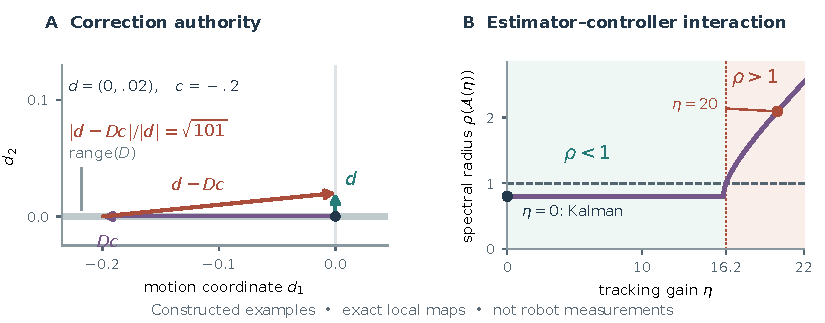
\includegraphics[width=\linewidth]{fig_theory_analysis.pdf}
\caption{\textbf{Two distinct barriers to repair in exact constructed models.}
(A) Restricting a full inverse to one input creates a large error: the permitted response
$Dc$ lies on the horizontal line, while $d$ has an unavailable component. The red arrow is
the remaining error; a constrained solve instead selects $c=0$.
(B) For the scalar model in Section~\ref{sec:analysis}, increasing composite tracking gain
eventually makes the augmented dynamics unstable although the healthy model and Kalman
observer are stable. The $16.2$ boundary belongs to this constant-gain, unclipped example;
it is not a robot tuning threshold.}
\label{fig:theory-analysis}
\end{figure}

\paragraph{Residual information and correction authority.}
Consider a noiseless residual $z=Hf$ and a physical discrepancy $Gf-Dc$, where $f$ is the
unknown disturbance and $c$ the permitted correction. Exact linear cancellation $c=Fz$
for every $f$ is possible precisely when
\begin{equation}\label{eq:main-factorization}
 \ker H\subseteq\ker G,\qquad \operatorname{range}(G)\subseteq\operatorname{range}(D).
\end{equation}
The first condition requires observing the disturbance components that matter physically;
the second requires sufficient input directions. Identifying all of $f$ is stronger than
the first condition and does not imply the second. With a bounded interface, the particular
response must also belong to $D\mathcal U$. Torque is matched relative to torque inputs;
configuration dependence alone does not imply unmatched uncertainty at another interface.
This characterization is Proposition~\ref{prop:authority}. A constant residual bias is likewise indistinguishable from a constant input fault without
outside information (Proposition~\ref{prop:sep}).

\paragraph{Inversion and input restriction need not commute.}
An exact full inverse can itself be harmful when followed by a mask
(Figure~\ref{fig:theory-analysis}A). For example, let
\[
 M=\begin{pmatrix}1&1\\0&.1\end{pmatrix},\qquad
 d=\begin{pmatrix}0\\.02\end{pmatrix},\qquad
 M^{-1}d=\begin{pmatrix}-.2\\.2\end{pmatrix}.
\]
If only the first input is available, applying $c=-.2$ gives physical error
$(.2,.02)^\top$, increasing its norm by $\sqrt{101}$. Allocation over that permitted column
instead chooses zero: the second direction is unavailable. This exact-model counterexample
motivates solving over permitted inputs rather than treating mask selection as an innocuous
final step. It explains a possible failure of the architecture, not the cause of a particular
Panda episode. Appendix~\ref{app:authority} also constructs full-authority harm from a small
map perturbation despite a $98\%$ reduction in the nominal objective.

\paragraph{A fitted objective is not a physical guarantee.}
Let $d$ be the physical disturbance response and suppose
$\|d-v\|_W\le\epsilon$ and $\|W^{1/2}(D-\widehat D)\|_2\le\zeta$. Then every candidate $c$
satisfies
\begin{equation}\label{eq:main-bound}
 \|d-Dc\|_W\le\|v-\widehat D c\|_W+\epsilon+\zeta\|c\|_2.
\end{equation}
Since $\|d\|_W\ge\|v\|_W-\epsilon$, a sufficient condition for improvement over zero
correction is a nominal residual reduction exceeding $2\epsilon+\zeta\|c\|_2$.
Proposition~\ref{prop:authority-certificate} also gives a bound on squared-error improvement
using the same physical baseline. The ridge solution improves its nominal objective because zero is feasible, but this alone
does not satisfy the physical condition. Calibration error and large inverse gains consume
the available improvement. Our experiments do not establish uniform bounds on $\epsilon$
and $\zeta$; the inequality is a conditional diagnostic, not an implemented safety gate.

\paragraph{Stable healthy dynamics do not make every composite gain stable.}
For the ideal matched position dynamics, with inactive clipping and constant fault, write
$\tilde\theta_t=\hat\theta_t-f$ and $\xi_t=(e_t,\tilde\theta_t)$. The actual update timing gives
\begin{equation}\label{eq:main-augmented}
 \xi_{t+1}=\mathcal A_t\xi_t+w_t,\qquad
 \mathcal A_t=\begin{bmatrix}A&-D\\T_tA&F_t-T_tD\end{bmatrix},
 \qquad F_t=d_\lambda(I-K_tM).
\end{equation}
$w_t$ collects model and measurement errors and, for nonzero damping, a constant-fault bias
term. If a \emph{single} $V\succ0$ satisfies
$\mathcal A_t^\top V\mathcal A_t\preceq\beta^2V$ for every realized gain, with $\beta<1$, then
\begin{equation}\label{eq:main-iss}
 \|\xi_t\|_V\le\beta^t\|\xi_0\|_V+
 \sum_{j=0}^{t-1}\beta^{t-1-j}\|w_j\|_V.
\end{equation}
Proposition~\ref{prop:composite-iss} proves this bound, including explicit forcing terms
for damping and model error. Tracking also multiplies model error by $T_t$, so increasing
feedback changes robustness as well as tracking. Individual frozen-gain
Schur tests do not establish a common metric or stability of arbitrary gain products.
Even in one dimension, $A=.8$, $D=M=L=1$, $K=P^+=.2$, $\Delta t=1$ and zero damping yield
a stable augmented matrix only for $0\le\eta<16.2$ (Figure~\ref{fig:theory-analysis}B);
$\eta=20$ destabilizes a stable healthy
model and Kalman observer. Extra tracking feedback therefore has no unconditional
superiority guarantee. Finally, converting a state-error bound into task success requires
a separate robustness assumption on a complete task trajectory; position RMS alone supplies
no such assumption.

\section{Experiments}
\label{sec:evaluation}
The experiments test the three links in the argument: does a calibrated residual support
repair at the command interface; does that repair extend when disturbances enter below the
controller; and does adding position feedback improve task success after observer tuning?
Historical evidence motivates the hypotheses, independent confirmations test their scope,
and physical/telemetry probes examine why aggregate scores can be misleading.
Detailed cells and diagnostics are in Appendix~\ref{sec:exp}.

\subsection{Evaluation design and scope}
New confirmations freeze configurations before evaluating untouched scenarios, restore
faults on every exit, verify complete physical initial states and source hashes, and
interleave arms with shared controls. Policy sampling remains independent: rescues and
regressions are observed paired differences, not deterministic counterfactuals. Historical
logs do not retrospectively certify these full-state checks. Newer GR1/WidowX cells (Appendix~\ref{sec:gr1}) are paired; older GR1 cohorts are not.
Per-cell paired tests use exact McNemar; repeated scenarios across fault conditions are
clustered for the estimator study's primary comparison. All declared comparison families
are retained, including harmful cells.

\textbf{Calibration separation.} The original LIBERO calibration protocol overlaps evaluated
task/initial-state combinations; its exact FIR scenario provenance is incomplete. We retain
those results as historical evidence, not fully held-out confirmation. The new Panda study
fits separate healthy calibrations per suite at initial states 25/26 and confirms at 35/36;
it does not test unchanged-calibration suite transfer. The ALOHA all-joint allocator reuses
historical sensitivity. The separate estimator study uses fresh healthy fit/qualification
seeds 3100--3129, search 3200--3203, validation 3300--3307 and confirmation 3400--3429.

\subsection{Calibrated residuals support command-interface repair}
The original $\pi_{0.5}$ experiment injects $+0.05$ on all six LIBERO action dimensions and
corrects rotation only, selected by faulted separation tests. Across Spatial/Goal/Object/10,
success is $28/120\to78/120$ (51 rescues, 1 regression, exact $p=2.35\times10^{-14}$);
all four suite tests survive Bonferroni-4; with the mask replaced by a healthy-data gate the
Spatial cell repeats at $9/20\to19/20$ (10 fixed, 0 broken, $p=0.002$; healthy control
$20/20\to19/20$). This motivates calibrated interface adaptation, subject to the caveat above. Original backbone-transfer and identify-then-hold
results remain in the appendix with their distinct protocols.

The selected Panda frames in Figure~\ref{fig:interface} illustrate this repair regime.
Their separate video protocol and outcome selection are documented in Appendix~\ref{app:videos}.


A matched-residual pilot yields 19, 17, 17, 18, 15 and 20 successes out of 20 for
the original observer, DOB, RLS, Kalman, calibrated integral and oracle, respectively.
Several estimators exploit the calibrated signal; the sample
does not establish equivalence or a unique benefit of the original update. By contrast, the
raw-error integral's $7/20$ versus calibrated $19/20$ changes the residual construction as
well as the update, so it cannot isolate either $M$ or the adaptive law.

\subsection{Physical-fault repair depends on the joint and task}
\begin{figure}[t]
\centering
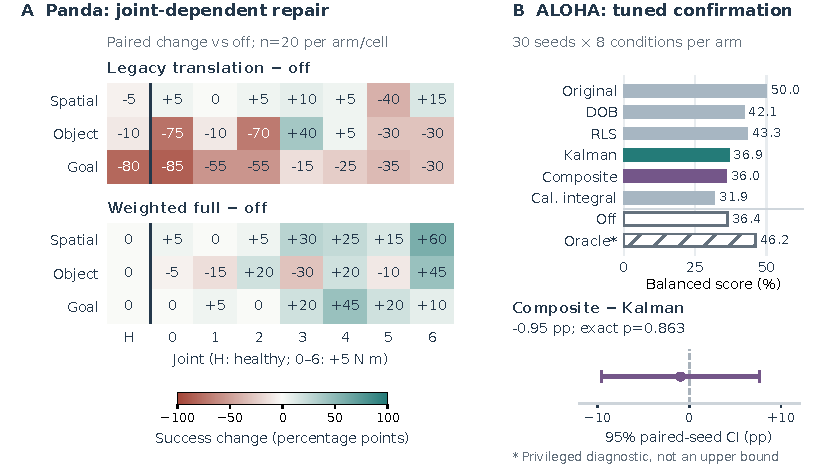
\includegraphics[width=\linewidth]{fig_results_analysis.pdf}
\caption{\textbf{Complete confirmation outcomes expose the scope of repair.}
(A) Paired success changes relative to shared correction-off controls for every Panda
suite and joint; $n=20$ per arm/cell and H denotes healthy. Colors show percentage-point
changes, not per-cell significance. (B) ALOHA balanced scores after frozen estimator
selection on 30 new seeds: half healthy success plus half the mean of seven fault rates.
The interval is the primary paired whole-seed bootstrap 95\% interval for composite minus
Kalman, with an exact sign-flip $p$-value. Scores do not establish a total ranking; oracle
is an unranked diagnostic.}
\label{fig:results-analysis}
\end{figure}

The historical seven-joint Panda map has equal overall totals, $103/140$ off and corrected,
but joint 5 falls $12/20\to3/20$ (Bonferroni-7 $p=.02734$). These are continuously updated,
translation-only corrections. We therefore tested correction support and regularization,
then froze a weighted-full candidate for independent confirmation.

The Panda confirmation uses frozen $\pi_{0.5}$ and comprises 1,440 rollouts: seven $+5$\,N\,m joint faults plus healthy,
three LIBERO suites, 20 scenarios per cell, and off/legacy translation/weighted full arms.
The $+5$\,N\,m injection is equal in torque, not in fractional actuator severity across joints.
The registered joint-5 primary improves legacy $15/60$ to weighted $41/60$ (29 rescues,
3 regressions, $p=2.556\times10^{-6}$). Off scores $36/60$, a descriptive secondary
comparison (Table~\ref{tab:main-physical}). Weighted full changes both correction support and regularization; it does not
isolate their individual effects.
\begin{table}[t]
\centering\small
\caption{Representative independent physical-fault results. Counts are successes; the last
column tests weighted against legacy, except the healthy Goal row, which tests off against
legacy. Adjustments use the stated family. Full allocations are in
Appendix~\ref{app:joint}. A significant improvement over a harmful comparator is not a
uniform-repair result.}
\label{tab:main-physical}
\begin{tabular}{lrrrl}
\toprule
condition & off & legacy & weighted & comparison \\
\midrule
Panda joint 5, three suites & 36/60 & 15/60 & 41/60 & primary $p=2.56\!\times\!10^{-6}$ \\
Panda Object, joint 3 & 8/20 & 16/20 & 2/20 & Bonf.-24 $p=.01245$ \\
Panda Goal, healthy & 19/20 & 3/20 & 19/20 & Bonf.-24 $p=.00073$ \\
ALOHA, all faulted cells & 60/240 & 70/240 & 66/240 & descriptive total \\
ALOHA, healthy & 11/20 & 8/20 & 6/20 & unresolved after Bonf.-13 \\
\bottomrule
\end{tabular}
\end{table}

The counterexample is Object joint 3: weighted drops legacy $16/20$ to $2/20$
(Bonferroni-24 $p=.01245$). Legacy also harms healthy Goal ($19/20$ off versus $3/20$
legacy). A separate 780-rollout ALOHA test covers all twelve arm joints plus healthy,
20 seeds and three arms under frozen $\pi_0$. No per-cell contrast resolves after Bonferroni-13; this establishes
neither transfer benefit nor equivalence. Healthy weighted falls from $11/20$ off to $6/20$.
The weighted variant remains experimental.

\textbf{What the complete joint map adds.} Figure~\ref{fig:results-analysis}A shows
numerical gains over off in 14 of 24 weighted-full cells and losses in four, compared with
seven gains and sixteen losses for legacy translation. These are descriptive cell counts,
including healthy conditions. The remaining weighted losses all occur on Object, while
Goal changes from uniformly negative legacy differences to nonnegative weighted differences.
Thus changing the permitted correction and its allocation can substantially broaden the
repair regime, but its effectiveness still depends on the task as well as the joint.
A net change of zero can contain both rescued and broken episodes. The shared off baseline
exposes this pattern; the prespecified primary statistical comparison remains weighted
versus legacy on joint 5, rather than a significance claim for every colored cell.

\textbf{Physical probes.} After observer initialization, legacy translation worsens local
scaled physical error in 150/168 Panda interventions and weighted full in 92/168, despite
all weighted solves satisfying their nominal objective checks. One candidate reduces its
model objective to 10.5\% of zero correction while increasing physical error in the same
covariance metric 2.69-fold. Conversely, privileged $-\tau/k_p$ shifts cancel all 144 tested
local ALOHA torque responses to numerical precision. These probes establish that local
authority can exist while the deployed estimate/allocation remains ineffective; they do not
identify every task failure's cause.

\subsection{Better composite tracking does not establish better task success}
We evaluate frozen $\pi_0$ (\code{pi0\_aloha\_sim}) on ALOHA Transfer Cube with left-six
correction at 50\,Hz, 300-step episodes and
ten-action chunks. Conditions are healthy, a $+0.02$\,rad offset on the six commands, and
torques $[16,32,16,.2,1,.4]$\,N\,m on individual left joints. The fitted six-position model
passes the declared $.005$-rad per-coordinate prediction gates (maximum rollout RMSE
$.00332$; fitted contraction factor $.895$). The twelve-joint reference fails qualification,
so the all-joint allocator experiment above is not a composite experiment.

The candidate bank contains 168 estimated recipes across six families, plus off and oracle;
seven composite candidates fail the fixed local screen. All 163 eligible arms enter search:
2,608 rollouts select two candidates per family, 896 validation rollouts select one, and
1,920 confirmation rollouts evaluate those six plus two controls on 30 untouched seeds.
The 5,424 total includes development, not 5,424 independent confirmation episodes.
Composite has a larger search pool; no settings are selected from confirmation outcomes.

\begin{table}[t]
\centering\small
\caption{Independent ALOHA estimator confirmation. The fixed score is half healthy success
plus half the mean of seven fault success rates. The ordering is numerical, not an
established ranking. All selected settings and individual cells are in Appendix~\ref{app:tuning}.}
\label{tab:main-estimators}
\begin{tabular}{lrrr}
\toprule
method/control & healthy & faulted & balanced score \\
\midrule
Original & 16/30 & 98/210 & 50.00\% \\
RLS & 17/30 & 63/210 & 43.33\% \\
DOB & 14/30 & 79/210 & 42.14\% \\
Kalman & 12/30 & 71/210 & 36.90\% \\
Composite & 12/30 & 67/210 & 35.95\% \\
Calibrated integral & 11/30 & 57/210 & 31.90\% \\
\midrule
Off & 15/30 & 48/210 & 36.43\% \\
Oracle (unranked) & 13/30 & 103/210 & 46.19\% \\
\bottomrule
\end{tabular}
\end{table}
Table~\ref{tab:main-estimators} and Figure~\ref{fig:results-analysis}B report the selected
configurations. The primary composite-minus-Kalman difference is $-0.95$ percentage points, with a
whole-seed bootstrap 95\% interval $[-9.52,7.62]$ and exact sign-flip $p=.86261$ under
whole-seed exchangeability/sign symmetry. None of four secondary overall Kalman contrasts
survives Holm correction. DOB beats Kalman on the offset cell ($9/30$ versus $0/30$,
Bonferroni-8 $p=.03125$ within that contrast's family). The oracle exactly cancels command
offsets but uses only nominal torque/$k_p$ compensation; independent policy sampling also
prevents interpreting its observed task score as an upper bound.

\begin{figure}[t]
\centering
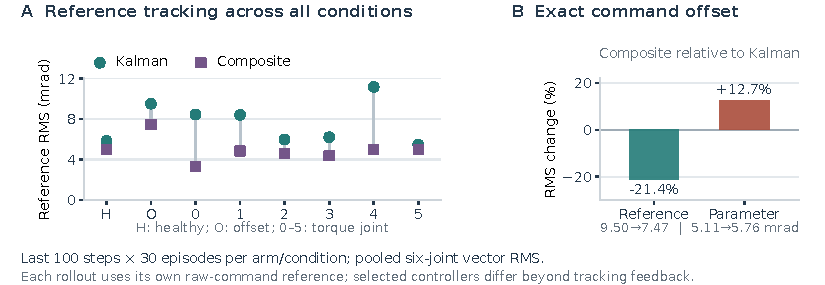
\includegraphics[width=\linewidth]{fig_tracking_analysis.pdf}
\caption{\textbf{Reference tracking and disturbance identification differ.}
(A) Pooled RMS norms over six joint positions in each rollout's final 100 steps,
30 episodes per arm/condition. Each reference follows that rollout's raw commands.
(B) On the known command offset, composite lowers reference error but raises parameter
error relative to Kalman. These selected controllers differ in bandwidth, damping and
clipping as well as tracking. The plot is descriptive and does not isolate tracking feedback.}
\label{fig:tracking-analysis}
\end{figure}

\textbf{Tracking is an incomplete success proxy.} Figure~\ref{fig:tracking-analysis}
separates reference tracking from known-offset identification. Over the last 100 steps, composite lowers
reference RMS in every confirmation condition, but over 99.39\% of its tracking-increment
energy on corrected coordinates lies on joint 1. On the exact-offset cell, reference RMS improves
from Kalman's $.00950$ to $.00747$\,rad while parameter RMS worsens from $.00511$ to
$.00576$\,rad, a 21.4\% decrease and 12.7\% increase. These are pooled six-coordinate vector
norms, not per-coordinate prediction RMSE; each controller follows its own raw-command
reference. Selected controllers also differ in bandwidth, damping and clipping, so these
diagnostics do not isolate the effect of tracking feedback (Appendix~\ref{app:tuning}).

\section{Limitations and implications}
\label{sec:limits}
The analysis is conditional on local maps, bounded mismatch and a common stability metric;
the current qualification checks do not certify the full nonlinear VLA--robot loop. The
physical-fault confirmations cover two robots, three LIBERO suites and one ALOHA task, while
the composite study covers only the left-six ALOHA interface. The finite tuning bank is not
a global optimum and omits a calibrated zero-process-noise static Kalman variant. Historical
calibration overlap limits the original transfer evidence, and old friction/lock efficacy
requires reruns with corrected fault cleanup. Hardware repair is pending; an unmodellable plant
(SimplerEnv's Google robot under base OpenVLA, $R^2=0.57$) is outside the method. Next:
state-dependent correction responses, calibration uncertainty, tracking isolated with identical
observer parameters.

\section{Conclusion}
Calibrated residuals enable frozen-policy repair in some command-interface settings; extending
that requires separating what can be inferred, what the inputs can change, and whether the
feedback is stable. Our conditions and confirmations make this testable: weighted allocation
repairs one joint while harming another, and composite tracking's advantage over Kalman is unresolved.
\label{main:lastpage}

\clearpage
\phantomsection\label{backmatter:firstpage}
\subsection*{AI use statement}
Generative AI (Claude, Anthropic; Codex, OpenAI) assisted with method and experiment design,
implementation, data analysis and interpretation, theoretical derivations and manuscript drafting. The authors are responsible for verifying
the final arguments, experimental claims and artifacts. Stored outcomes and reproducible
analysis, rather than generated explanations, support empirical claims.

\subsection*{Reproducibility statement}
The appendix provides full assumptions and proofs, implementation timing, calibrations,
selected parameters and per-condition counts. Supplementary artifacts include frozen
protocols, source/input hashes, complete allocated outcomes, independent statistical
cross-checks and telemetry diagnostics. Historical results with incomplete provenance are
explicitly separated from new confirmations. No physical-fault or estimator confirmation
outcomes were used to revise their frozen candidates.

\bibliography{refs}
\bibliographystyle{iclr2027_conference}
\clearpage
\appendix
\section{Conditional theory for interface repair}
\label{app:composite-theory}

This appendix separates algebraic identifiability, the authority of the chosen
action interface, and stability of the implemented observer. Its dynamical
results concern an explicitly assumed local model. They do not turn the fitted
healthy reference or the reported per-step eigenvalue screens into a certificate
for the physical VLA--robot loop.

\subsection{Identifying a disturbance is different from cancelling its effect}

Let a constant parameter $f\in\mathbb R^p$ produce a bias-corrected observation
$z=Hf$ and an unwanted physical response $Gf\in\mathbb R^n$. A correction
$c\in\mathbb R^k$ removes the response $Dc$, where $D\in\mathbb R^{n\times k}$
describes the available action interface. Thus $H$ describes observation and $D$
describes correction authority; neither is assumed equal to $G$.

\begin{proposition}[Identifiability and exact linear cancellation]
\label{prop:authority}
The parameter $f$ is uniquely identifiable from $z$ if and only if
$\ker H=\{0\}$. There exists a linear rule $c=Fz$ cancelling every parameter,
$DFH=G$, if and only if
\begin{equation}\label{eq:authority-factorization}
\ker H\subseteq\ker G,\qquad
\operatorname{range}G\subseteq\operatorname{range}D.
\end{equation}
With corrections restricted to a set $\mathcal U$, exact cancellation for a
particular known $f$ is feasible if and only if $Gf\in D\mathcal U$.
\end{proposition}
\begin{proof}
Two parameters yield the same observation exactly when their difference lies
in $\ker H$, proving the first assertion. If $DFH=G$, then $Hv=0$ implies
$Gv=0$, and every column of $G$ lies in the range of $D$, proving necessity.
Conversely, let $H^\dagger,D^\dagger$ denote Moore--Penrose inverses. The two
conditions give $GH^\dagger H=G$ and $DD^\dagger G=G$, respectively. Therefore
$F=D^\dagger GH^\dagger$ satisfies $DFH=G$. The bounded assertion is precisely
the existence of $c\in\mathcal U$ with $Dc=Gf$.
\end{proof}

Full parameter identifiability is consequently neither sufficient nor necessary
for cancellation of the physical effect. For example, $H=I_2$, $G=I_2$ and
$D=(1,0)^\top$ make both fault coordinates observable while leaving the second
uncorrectable. Conversely, $H=(1,0)$, $G=(1,0)$ and $D=1$ permit exact cancellation
although the irrelevant second fault coordinate is unidentifiable. These are
local interface statements: configuration dependence alone establishes neither
of the range conditions. Unknown output bias further limits identifiability as
in Proposition~\ref{prop:sep}.

\subsection{The recursion implemented by the composite observer}

For the following result the estimate and fault have the same $p$ coordinates.
Suppose that, over a stated operating region, actual-minus-reference position
error obeys
\begin{equation}\label{eq:local-position-error}
e_{t+1}=Ae_t+Gf_t-D\hat\theta_t+w_{t+1},\qquad
z_{t+1}=Hf_t+v_{t+1}.
\end{equation}
Here $w$ includes model error and $v$ includes observation error, remaining bias,
and any discrepancy in the calibrated residual relation. Cancellation by the
estimate $\hat\theta=f$ requires $(G-D)f=0$, for example when $G=D$ or the
admissible faults occupy only coordinates where the two maps agree. The more
general authority condition in Proposition~\ref{prop:authority} can instead
require a different allocation of the identified parameter. For ALOHA,
$H=M$ is the full residual sensitivity,
$D=B\operatorname{diag}(m)$ includes the correction mask, and the fitted reference
is driven by the live \emph{raw} action. Subtracting this reference cancels the
common raw input in the assumed linear model; it does not construct the healthy
counterfactual trajectory of the nonlinear policy.
Using the fitted $D$ in the physical recursion is an assumption: if the actual
map is $D_{\rm phys}$, the remainder must include
$-(D_{\rm phys}-D)\hat\theta_t$. Applying the bounds below then requires a
bound on this remainder over the operating region; fitting $D$ does not supply
that bound automatically.

Write $a=\exp(-\lambda\Delta t)$ and
$h=\Delta t$ when $\lambda=0$, otherwise $h=(1-a^2)/(2\lambda)$.
The implementation uses
\begin{align}
P_t^-&=a^2P_t+hQ_c,
&K_t&=P_t^-H^\top(HP_t^-H^\top+R)^{-1},\\
P_t^+&=(I-K_tH)P_t^-(I-K_tH)^\top+K_tRK_t^\top,
&P_{t+1}&=P_t^+,\\
T_t&=\Delta t\,\eta P_t^+D^\top L,
&\bar\theta_{t+1}&=a\hat\theta_t+K_t(z_{t+1}-Ha\hat\theta_t)+T_te_{t+1},\\
\hat\theta_{t+1}&=\Pi_{\mathcal U}(\bar\theta_{t+1}).&&
\label{eq:appendix-composite-recursion}
\end{align}
Here $Q_c$ is process covariance per unit time, $R\succ0$ is covariance per
observation, and $L\succ0$ is the chosen position metric. The action has already
used $\hat\theta_t$ before $e_{t+1}$ and $z_{t+1}$ are measured. $P_t^+$ is the
posterior covariance of the specified prediction-only statistical model; after
adding tracking feedback it is a design preconditioner, not automatically the
true covariance of the composite estimation error.

Let $\delta_t=\hat\theta_t-f_t$, $C_t=I-K_tH$, and
$\xi_t=(e_t^\top,\delta_t^\top)^\top$. Define
\begin{align}
b_{t+1}&=(G-D)f_t+w_{t+1},
&\Delta f_t&=f_{t+1}-f_t,\\
p_{t+1}&=\Pi_{\mathcal U}(\bar\theta_{t+1})-\bar\theta_{t+1}.
\end{align}
Direct substitution yields the exact error recursion under
\eqref{eq:local-position-error}:
\begin{equation}\label{eq:composite-augmented}
\begin{aligned}
\xi_{t+1}&=\mathcal A_t\xi_t+d_{t+1},\\
\mathcal A_t&=
\begin{bmatrix}
A&-D\\
T_tA&aC_t-T_tD
\end{bmatrix},\\
d_{t+1}&=
\begin{bmatrix}
b_{t+1}\\
T_tb_{t+1}+(a-1)C_tf_t-\Delta f_t+K_tv_{t+1}+p_{t+1}
\end{bmatrix}.
\end{aligned}
\end{equation}
In particular, the lower-left block is $T_tA$, not $T_t$: tracking uses the
\emph{new} position error. The positive tracking sign is also deliberate. For
fixed $e_t,f_t$, the gradient of
$\frac12\|Ae_t+Gf_t-D\theta\|_L^2$ at $\theta=\hat\theta_t$, in the noiseless
model, is $-D^\top Le_{t+1}$. Hence tracking alone is a preconditioned negative
gradient step. This direction does not establish stability of the full finite-step
observer--controller recursion.

\begin{proposition}[Conditional contraction and disturbance bound]
\label{prop:composite-iss}
Assume \eqref{eq:local-position-error} holds along the trajectory. Suppose a
\emph{single} matrix $V\succ0$ and $0<\rho<1$ satisfy
\begin{equation}\label{eq:common-composite-metric}
\mathcal A_t^\top V\mathcal A_t\preceq\rho^2 V
\quad\text{for every gain encountered.}
\end{equation}
Then, with $\|x\|_V=(x^\top Vx)^{1/2}$,
\begin{equation}\label{eq:composite-iss-bound}
\|\xi_t\|_V
\le \rho^t\|\xi_0\|_V+
\sum_{s=0}^{t-1}\rho^{t-1-s}\|d_{s+1}\|_V.
\end{equation}
If $\|d_{t+1}\|_V\le\bar d$, the second term is at most
$\bar d(1-\rho^t)/(1-\rho)$. For a constant fault with $(G-D)f=0$,
zero damping, no model or observation error, and inactive projection, the
origin converges exponentially.
\end{proposition}
\begin{proof}
To obtain \eqref{eq:composite-augmented}, first substitute
$\hat\theta_t=\delta_t+f_t$ into the position equation. For the parameter equation,
subtract $f_{t+1}$ from the update. The coefficient of $f_t$ is
$aC_t+K_tH-I=(a-1)C_t$, and substituting the new position equation supplies
$T_tA$, $-T_tD$ and $T_tb_{t+1}$. Projection adds exactly $p_{t+1}$.
Under \eqref{eq:common-composite-metric},
$\|\mathcal A_t x\|_V\le\rho\|x\|_V$. The triangle inequality followed by
induction proves \eqref{eq:composite-iss-bound}; summing the geometric series
proves the uniform-input bound. In the last stated case every forcing term is
zero.
\end{proof}

Projection cannot simply be dropped from this argument: Euclidean box projection
need not be nonexpansive in a metric with position--parameter cross terms.
One sufficient extension is $V=\operatorname{diag}(V_e,cI_p)$ with $c>0$ and
$f_{t+1}\in\mathcal U$, where $\mathcal U$ is the implemented closed convex box.
Then
$\|\Pi_{\mathcal U}(\bar\theta)-f_{t+1}\|_2
\le\|\bar\theta-f_{t+1}\|_2$, so the same bound holds with the projection term
omitted from $d$, provided the common-metric inequality holds for this block
metric. For a general $V$, a separate bound on $p$ is needed.

For fixed gains, a Schur $\mathcal A$ admits a quadratic contraction metric.
For changing gains, checking each matrix separately is insufficient. For example,
$\left[\begin{smallmatrix}.5&2\\0&.5\end{smallmatrix}\right]$ and
$\left[\begin{smallmatrix}.5&0\\2&.5\end{smallmatrix}\right]$ each have spectral
radius $.5$, but their two-step product has spectral radius $2.25+\sqrt5>1$.
This example is a general switching counterexample, not an assertion that these
two matrices occur in our experiments. The existing candidate screen checks
frozen augmented matrices over the covariance transient and at its limit; it
does not verify \eqref{eq:common-composite-metric}, even for that finite horizon.
Likewise, a fitted $A$ satisfying $A^\top LA\prec L$ need not make the augmented
system contractive. The proposition is conditional on additional, computable
matrix inequalities and valid model/error bounds.

\paragraph{Damping introduces forcing.}
For a constant fault with $(G-D)f=0$, $w=v=p=0$ and fixed gains, positive damping
leaves $d=(0,((a-1)Cf)^\top)^\top$. If $\mathcal A$ is Schur, then
\begin{equation}\label{eq:damped-equilibrium}
\xi_*=(I-\mathcal A)^{-1}
\begin{bmatrix}0\\(a-1)Cf\end{bmatrix}.
\end{equation}
Thus stability generally gives a biased equilibrium rather than exact fault
cancellation. For the scalar prediction-only case $H=1$, $K=k$, $T=0$,
\begin{equation}
\hat\theta_* = \frac{k}{1-a(1-k)}f.
\end{equation}
For $0<k<1$ and $0<a<1$ this attenuates a nonzero fault. With zero damping,
fixed-gain Kalman is the $T=0$ special case; equality of algorithms requires
matching $Q_c,R,P_0$ and projection as well.

\begin{proposition}[Positive tracking gain can destabilize a stable observer]
\label{prop:tracking-limit}
There are an exactly matched scalar plant with contractive healthy dynamics and
valid steady Kalman covariances for which increasing positive tracking gain
destabilizes the implemented local composite recursion.
\end{proposition}
\begin{proof}
Take $A=.8$, $G=D=H=L=1$, $\lambda=0$, $\Delta t=1$, $R=1$, $Q_c=.05$ and
$P_t=P_t^+=.2$. Then $P_t^-=.25$, $K_t=.2$, and $T_t=.2\eta$, all exactly
consistent with the covariance recursion. For inactive projection,
\begin{equation}
\mathcal A(\eta)=
\begin{bmatrix}.8&-1\\.16\eta&.8-.2\eta\end{bmatrix},\qquad
\operatorname{tr}\mathcal A=1.6-.2\eta,\quad
\det\mathcal A=.64.
\end{equation}
The second-order Schur conditions
$1-\det\mathcal A>0$, $1-\operatorname{tr}\mathcal A+\det\mathcal A>0$ and
$1+\operatorname{tr}\mathcal A+\det\mathcal A>0$ hold, for $\eta\ge0$, precisely
when $\eta<16.2$. Kalman alone ($\eta=0$) is stable, whereas $\eta=20$ gives
eigenvalues $-1.2\pm\sqrt{.8}$, one of magnitude greater than one. The same
local instability holds around the zero-fault equilibrium with any positive
box bound, since projection is inactive in a neighborhood of that equilibrium.
\end{proof}

The threshold is for this scalar example's rate $\eta$ and unit time step; it
is not a threshold for the ALOHA rate or its dimensionless active-strength setting.
This counterexample concerns the algorithm class; it is not a diagnosis of the
screened experimental configurations. Even within a stable range, the extra
term can introduce sensitivity to reference-model error or redistribute gains
across coordinates. Neither a positive gradient direction nor an empirical
contraction check implies a universal advantage over Kalman or the other
estimators.

\subsection{What would permit a task-success conclusion?}

\begin{proposition}[Transfer through an assumed robust trajectory tube]
\label{prop:task-tube}
Fix a successful nominal complete execution $x^0_{0:N}$. Suppose every execution
with $\max_{t\le N}\|x_t-x_t^0\|\le\epsilon_{\rm task}$ also succeeds.
Suppose, independently, the full-execution discrepancy satisfies
$\|x_t-x_t^0\|\le c\|\xi_t\|_V+\epsilon_{\rm lift}$ for all $t\le N$, and
the assumptions of Proposition~\ref{prop:composite-iss} hold with
$\|d_t\|_V\le\bar d$. Then the corrected execution succeeds whenever
\begin{equation}
c\max\!\left\{\|\xi_0\|_V,\frac{\bar d}{1-\rho}\right\}
+\epsilon_{\rm lift}\le\epsilon_{\rm task}.
\end{equation}
\end{proposition}
\begin{proof}
The bound in \eqref{eq:composite-iss-bound} is at most a convex combination of
$\|\xi_0\|_V$ and $\bar d/(1-\rho)$, hence no larger than their maximum.
The assumed lifting inequality places the complete execution in the successful
tube.
\end{proof}

Both additional assumptions are substantive. The complete execution must include
the variables needed to determine success; a six-position error does not bound
unobserved velocities, contact states, other joints, or changes in the policy's
observations. The fitted reference driven by each rollout's own raw actions is
also not the common successful nominal execution assumed here. Neither the
robust tube nor the lifting bound was established by our experiments. This
conditional result therefore states what is missing for task-level transfer,
not a success guarantee or a claim that any estimator must rank first.

% Compact main-text version (notation and complete proofs are below):
% At a fixed state and horizon, write e(c)=d-Dc. For a residual proxy v,
% nominal map Dhat, and bounds ||d-v||_R<=delta and
% ||R^{-1/2}(D-Dhat)||_2<=epsilon, let c minimize the box-constrained
% ridge objective. Put eta=epsilon||c||_2 and
% Delta=||v||_R^2-||v-Dhat*c||_R^2. Then physical squared-error reduction
% is at least Delta-2*eta*||v-Dhat*c||_R-eta^2
% -2*delta*(||Dhat*c||_R+eta). Positivity certifies local improvement
% under the stated uncertainty bounds, not task recovery; these bounds
% are not estimated or certified by the implemented allocator.

\section{Finite-horizon correction authority and model mismatch}
\label{app:authority}

This appendix separates three quantities: a measured residual, the physical
error it is intended to represent, and the response to an available correction.
The results concern a fixed initial state, nominal input sequence, disturbance,
and observation horizon. They are finite-dimensional statements, not stability
or task-success theorems.

Write the physical error relative to the corresponding healthy response as
\begin{equation}
 e(c)=d-Dc,\qquad d\in\mathbb R^m,\quad D\in\mathbb R^{m\times p},
 \qquad c\in\mathcal C:=\{c:|c_i|\leq\kappa_i\},\quad \kappa_i>0.
 \label{eq:authority-physical-map}
\end{equation}
The controller applies the negative of $c$ in the $p$ permitted input
coordinates. The vector $d$ may be written $Gf$ when a physical fault map $G$
and fault parameters $f$ are available. The matrix $D$ describes correction
authority; it is distinct from a fault-to-observation matrix $H$. In
particular, identifying $Hf$ does not establish that it equals $d$ or that
$d$ is cancelable through $D$.

Let $R\succ0$, set $W_R=R^{-1/2}$, and define
$\|x\|_R:=\|W_R x\|_2$; thus the subscript $R$ denotes the inverse-covariance
norm, $\|x\|_R^2=x^\top R^{-1}x$. An inverse Cholesky factor gives the same
norm and all results below. Input coordinates and their units are fixed when
using $\|c\|_2$. A change of input scaling must also change $D$ and the
operator-norm uncertainty bound.

\begin{proposition}[The available-input authority floor]
\label{prop:authority-floor}
Let $\Pi_D=(W_R D)(W_R D)^\dagger$ be the Euclidean orthogonal projector onto
$\operatorname{range}(W_R D)$. Then
\begin{align}
 \inf_{c\in\mathbb R^p}\|d-Dc\|_R^2
   &=\|(I-\Pi_D)W_R d\|_2^2, \label{eq:authority-projection-floor}\\
 \min_{c\in\mathcal C}\|d-Dc\|_R^2
   &=\|(I-\Pi_D)W_R d\|_2^2
     +\min_{c\in\mathcal C}\|\Pi_D W_R d-W_R Dc\|_2^2.
     \label{eq:authority-box-floor}
\end{align}
Consequently, exact cancellation with bounded permitted inputs is possible
if and only if $d\in D\mathcal C$. Perfect identification of $d$ alone does
not remove either the missing-direction floor or the bound-induced floor.
\end{proposition}

\begin{proof}
For every $c$, $W_R Dc$ lies in $\operatorname{range}(W_R D)$. Hence
\[
 W_R d-W_R Dc=(I-\Pi_D)W_R d+(\Pi_D W_R d-W_R Dc)
\]
is an orthogonal decomposition. Taking squared norms gives the identity
underlying both displays. Over $\mathbb R^p$, the second term attains zero,
for example at $c=(W_R D)^\dagger W_R d$. Over $\mathcal C$, it attains a minimum
because $\mathcal C$ is compact and the objective is continuous. The total
minimum is zero exactly when some $c\in\mathcal C$ satisfies $W_R Dc=W_R d$;
$W_R$ is invertible, so this is equivalent to $Dc=d$.
\end{proof}

The weighted allocator instead has a nominal map $\widehat D$ and a filtered
residual proxy $v$. With prior scales
$S=\operatorname{diag}(\sigma_1,\ldots,\sigma_p)\succ0$, its ideal numerical
solution is
\begin{equation}
 \widehat c=\mathop{\arg\min}_{c\in\mathcal C}J(c),\qquad
 J(c):=\|v-\widehat D c\|_R^2+\|S^{-1}c\|_2^2.
 \label{eq:authority-ridge}
\end{equation}
In the implementation, $v$ is the filtered, optionally bias-corrected FIR
residual and $\widehat D$ consists of the permitted columns of $M$. This
identifies the optimization actually performed. It does \emph{not} identify
$M$ with the physical correction map $D$ in
\eqref{eq:authority-physical-map}.

\begin{proposition}[Conditional physical improvement from a nominal allocator]
\label{prop:authority-certificate}
Suppose \eqref{eq:authority-physical-map} holds and
\begin{equation}
 \|d-v\|_R\leq\delta,\qquad
 \|W_R(D-\widehat D)\|_2\leq\varepsilon,
 \qquad \delta,\varepsilon\geq0.
 \label{eq:authority-uncertainty}
\end{equation}
For any fixed feasible candidate $c$, define
\[
 a=W_R v,\quad b=W_R\widehat D c,\quad q=\|c\|_2,\quad
 \eta=\varepsilon q,\quad
 \Delta(c)=\|a\|_2^2-\|a-b\|_2^2.
\]
Then
\begin{align}
 \|e(c)\|_R &\leq \|a-b\|_2+\delta+\eta,
   \label{eq:authority-error-envelope}\\
 \|d\|_R^2-\|e(c)\|_R^2
 &\geq \Delta(c)-2\eta\|a-b\|_2-\eta^2
             -2\delta(\|b\|_2+\eta).
   \label{eq:authority-improvement-certificate}
\end{align}
Strict positivity of the right-hand side of
\eqref{eq:authority-improvement-certificate} guarantees physical error
reduction for every $(d,D)$ satisfying \eqref{eq:authority-uncertainty}.
For the unique ridge minimizer in \eqref{eq:authority-ridge},
\begin{equation}
 \Delta(\widehat c)\geq\|S^{-1}\widehat c\|_2^2.
 \label{eq:authority-nominal-guarantee}
\end{equation}
This last inequality is a nominal guarantee and does not by itself imply
physical improvement when $\delta$ or $\varepsilon$ is nonzero.
\end{proposition}

\begin{proof}
Let $u=W_R(d-v)$ and $h=W_R(D-\widehat D)c$. The assumptions imply
$\|u\|_2\leq\delta$ and $\|h\|_2\leq\varepsilon\|c\|_2=\eta$.
Since $W_R e(c)=a-b+u-h$, the triangle inequality proves
\eqref{eq:authority-error-envelope}.

To compare against the \emph{same} physical baseline $d$, expand the
squared-error improvement before bounding the terms:
\begin{align*}
 \|W_R d\|_2^2-\|W_R e(c)\|_2^2
 &=\|a+u\|_2^2-\|a+u-b-h\|_2^2\\
 &=\Delta(c)+2(a-b)^\top h-\|h\|_2^2
                      +2u^\top(b+h)\\
 &\geq\Delta(c)-2\|a-b\|_2\eta-\eta^2
                      -2\delta(\|b\|_2+\eta).
\end{align*}
The last step uses Cauchy--Schwarz and $\|b+h\|_2\leq\|b\|_2+\eta$.
This proves \eqref{eq:authority-improvement-certificate} without treating
the baseline and corrected uncertainties as independent errors.

The ridge objective is continuous and strictly convex: its Hessian is
$2\widehat D^\top R^{-1}\widehat D+2S^{-2}\succ0$.
The compact convex box therefore contains a unique minimizer. Because zero
is feasible, $J(\widehat c)\leq J(0)=\|W_R v\|_2^2$. Rearranging yields
\eqref{eq:authority-nominal-guarantee}.
\end{proof}

\paragraph{Sharpness and an exact special-case threshold.}
For a fixed $c$, the upper bound in
\eqref{eq:authority-error-envelope} is attained by some admissible $(d,D)$.
For $c\ne0$, choose a unit vector $w$ parallel to $a-b$ (arbitrary when
$a=b$), put $W_R(d-v)=\delta w$, and choose the rank-one perturbation
\[
 W_R(D-\widehat D)=-\varepsilon w\frac{c^\top}{\|c\|_2}.
\]
Its operator norm is $\varepsilon$ and its product with $c$ is $-\eta w$,
so all three terms of $W_R e(c)$ align. If $c=0$, only the vector uncertainty
is needed. Thus, when the physical disturbance is known exactly ($v=d$)
and $c\ne0$, uniform strict improvement over the operator-norm ball is
equivalent to
\begin{equation}
 \|v-\widehat D c\|_R+\varepsilon\|c\|_2<\|v\|_R.
 \label{eq:authority-sharp-threshold}
\end{equation}
In particular, a nominal residual decrease must exceed the uncertainty
amplified by the chosen correction norm. A projection bound limits this
amplification to $\varepsilon\|\kappa\|_2$, but does not make it zero.

\paragraph{Numerical and nonlinear qualifications.}
The implementation checks box feasibility, KKT residuals, and its objective
against the zero-feasible objective up to numerical tolerance. For any
returned feasible candidate satisfying $J(c)\leq J(0)+\tau_{\rm opt}$,
the exact replacement for \eqref{eq:authority-nominal-guarantee} is
$\Delta(c)\geq\|S^{-1}c\|_2^2-\tau_{\rm opt}$; the physical inequalities
remain valid for that candidate without assuming exact optimality.
If a local nonlinear response is instead
$e(c)=d-Dc+\xi(c)$ with a separately justified
$\|\xi(c)\|_R\leq\nu(c)$, the error envelope acquires $+\nu(c)$.
Consequently, $\|v-\widehat D c\|_R+\delta+\varepsilon\|c\|_2+\nu(c)
<\|v\|_R-\delta$ is sufficient for strict physical improvement.
No such conclusion follows outside the region where these bounds hold.
The present allocator does not estimate or certify $\delta$, $\varepsilon$,
or $\nu$. A healthy residual covariance provides a weighting matrix; it is
not a uniform bound on these physical uncertainties.

\paragraph{Counterexample 1: identify first and mask afterward.}
Take $R=I$,
\[
 M=\begin{pmatrix}1&1\\0&0.1\end{pmatrix},\qquad
 d=\begin{pmatrix}0\\0.02\end{pmatrix},\qquad
 M^{-1}d=\begin{pmatrix}-0.2\\0.2\end{pmatrix}.
\]
Suppose only the first input can be corrected. Then $D=(1,0)^\top$ and
the authority floor is $\|d\|_2=0.02$. Applying the first component of the
full inverse gives $c=-0.2$, hence
$e(c)=(0.2,0.02)^\top$ and $\|e(c)\|_2/\|d\|_2=\sqrt{101}$.
All components fit inside a $0.3$ box. In contrast, allocation using the
permitted column gives $c=0$, with or without positive ridge. Thus even
an exact full inverse does not justify inverting and then masking.

\paragraph{Counterexample 2: a nearly correct map can give the wrong intervention.}
Here the disturbance proxy is exact, both physical directions are available,
and the actual box-constrained authority floor is zero. Set
\[
 \alpha=\frac1{100},\quad t=\frac15,\quad \tau=\frac1{100},
 \quad \lambda=\tau\alpha^2=10^{-6},
\]
\[
 \widehat D=\begin{pmatrix}1&1\\0&\alpha\end{pmatrix},\quad
 D=\begin{pmatrix}1&1+2\alpha\\0&\alpha\end{pmatrix},\quad
 v=d=\begin{pmatrix}0\\t\alpha\end{pmatrix}.
\]
Use $\mathcal C=[-0.3,0.3]^2$, $S=0.1I$, and
$R=10^{-8}I=0.01\lambda I$. Multiplication by $10^{-8}$ converts
\eqref{eq:authority-ridge} into
$\|v-\widehat D c\|_2^2+\lambda\|c\|_2^2$ without changing its minimizer.
Writing $Z=1+2\tau+\tau(1+\tau)\alpha^2$, its unconstrained minimizer is
\begin{equation}
 \widehat c=\frac{t}{Z}
             \begin{pmatrix}-1\\1+\tau\alpha^2\end{pmatrix}
 \approx\begin{pmatrix}-0.19607824\\0.19607843\end{pmatrix}.
 \label{eq:authority-counterexample-candidate}
\end{equation}
Both bounds are inactive, so this is also the unique box-constrained
minimizer. Direct substitution gives
\begin{align}
 \frac{J(\widehat c)}{J(0)}
 &=\frac{2\tau+\tau^2\alpha^2}{Z}
   =0.01960783\ldots<0.02,\\
 \frac{\|d-D\widehat c\|_R}{\|d\|_R}
 &=\frac{\sqrt{[2(1+\tau\alpha^2)+\tau\alpha]^2
                     +(2\tau+\tau^2\alpha^2)^2}}{Z}
   =1.9609804\ldots>1.96.
 \label{eq:authority-counterexample-harm}
\end{align}
For completeness, \eqref{eq:authority-counterexample-candidate} follows
by solving
\[
 \begin{pmatrix}1+\lambda&1\\1&1+\alpha^2+\lambda\end{pmatrix}
 \widehat c=\begin{pmatrix}0\\t\alpha^2\end{pmatrix},
\]
whose determinant is $\alpha^2Z$. At this stationary point the normalized
objective is $1-(1+\lambda)/Z$, giving the first ratio. The two physical
error coordinates divided by $t\alpha$ are
$-[2(1+\tau\alpha^2)+\tau\alpha]/Z$ and
$(2\tau+\tau^2\alpha^2)/Z$, proving the second ratio.

There is no sign reversal in the maps: their diagonals agree and are
positive, and only one positive cross-coupling changes. Moreover,
$\|D-\widehat D\|_2=0.02$ and
$\|D-\widehat D\|_2/\|\widehat D\|_2<0.02/\sqrt2<1.415\%$.
The actual exact correction $c_*=(-(1+2\alpha)t,t)^\top=(-0.204,0.2)^\top$
is feasible and satisfies $Dc_*=d$. Nevertheless, the nominal ridge
objective decreases by more than $98\%$ while physical error nearly doubles.
The small singular direction and cancellation between correction components
make an apparently small map error consequential. These are constructed
numbers, not fitted robot parameters or a causal reconstruction of a recorded
task failure.

The geometric floor concerns the chosen observed physical coordinates.
Cancellation of a six-dimensional endpoint error, for example, does not
establish cancellation of every coordinate of a seven-joint robot. Likewise,
even a valid finite-horizon physical-improvement bound does not establish
recovery of a task after an earlier trajectory error or guarantee repeated
closed-loop adaptation.

\section{Video illustrations and provenance}\label{app:videos}
Figure~\ref{fig:video-evidence} retains the complete paired Panda illustration.
Its source video is the documented camera-corrected re-render: recording and policy views
are separated and the residual uses SO(3) increments. Both panels display step 162, before
that step's environment transition; the success annotation describes its result. The
uncorrected rollout later times out at step 229. The clip was selected by observed outcome;
policy randomness was not pinned and full-state/initial-state identifiers were not archived.
It therefore supplies a visual example rather than an additional benchmark sample.

The ALOHA image in Figure~\ref{fig:interface} comes from a different video protocol:
a $+0.02$\,rad offset on left-arm commands 0--5, with a correction identified in one episode
and then held. It is a selected success from that held-correction experiment. The original
video's generic ``online'' banner does not describe this mode; the manuscript labels it
as held correction. The joint-5 failure panel instead reads the stored 20-episode torque
cell directly. Its $+5$\,N\,m torque and continuous translation-only correction differ from
both video conditions. Source frames, exact crops and SHA-256 hashes accompany the figure
reproduction scripts. Scenes are exact crops of recorded frames.

\begin{figure}[t]
\centering
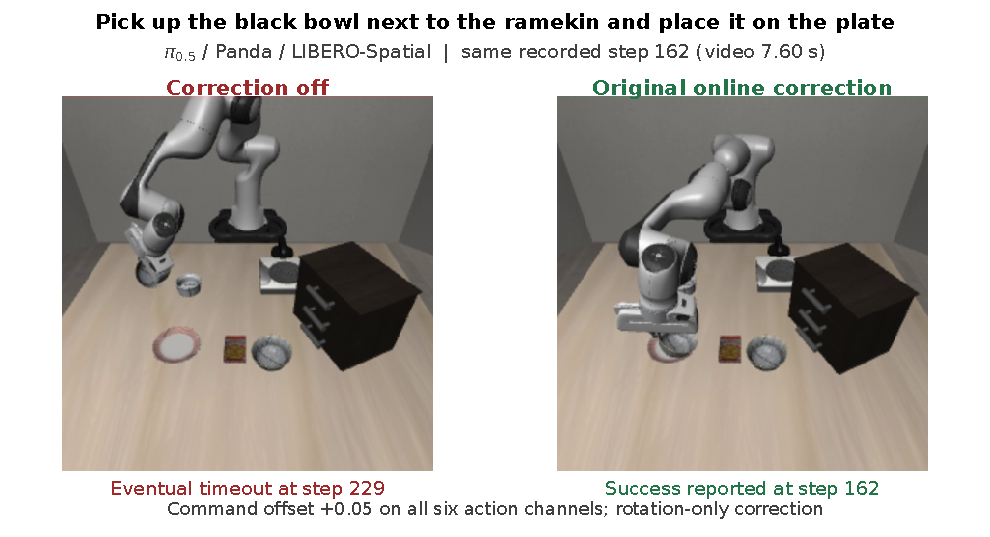
\includegraphics[width=.88\linewidth]{fig_video_evidence.pdf}
\caption{Selected video demonstration: frozen $\pi_{0.5}$ on LIBERO-Spatial, with
$+0.05$ offsets on all six motion-action channels and online rotation-only correction.
Both images are from displayed step 162. The corrected run reports success on the
transition following this rendered frame; the uncorrected run later times out at step 229.
The task is to place the black bowl next to the ramekin onto the plate. This historical
illustration is separate from the confirmation counts and the composite--Kalman comparison.}
\label{fig:video-evidence}
\end{figure}

\section{Implementation details}\label{app:implementation}
\paragraph{Recorded adapter behavior.}\label{app:adapterstate}
In the tested original $\pi_{0.5}$ LIBERO adapter, zeroing the state input produced no
recorded action change (reported difference $0.00000$). This concerns that input path;
it does not exclude visual feedback or compensation by the policy.

\label{sec:method}

\subsection{Plant, residual, and sensitivity}

On healthy rollouts we identify a per-channel FIR plant
\begin{equation}
\hat y_t = \sum_{\ell=0}^{K} h_\ell\, u_{t-\ell} + c, \qquad K = 6,
\end{equation}
where $u_t$ is the command we \emph{believe} we sent (the policy's action plus any
correction we applied). For LIBERO the plant predicts the increment; for ALOHA it predicts
the position, because there the command is an absolute target that a servo tracks and a
target offset lives in the steady-state position error, not in the increment
(\S\ref{sec:aloha}). The residual
\begin{equation}
r_t = y_t - \hat y_t
\end{equation}
is what the healthy plant cannot explain. Because $u_t$ includes the correction and the
world executes $u_t + f$, a local linear approximation gives $r_t \approx M f$ and hence
an estimate of the \emph{total} fault. Correction-dependent model error, contacts and torque
faults can violate this approximation. $M = \partial(\text{motion})/\partial(\text{fault})$ is a
$d\times d$ sensitivity matrix measured once by open-loop replay: a recorded healthy command
sequence is replayed with and without a per-axis probe, and the mean motion difference per
unit probe gives each column. On the LIBERO plant $M$ is diagonal-dominant with
$\mathrm{cond}(M)=3.0$ and is magnitude independent to within $14\%$ between probes of
$0.02$ and $0.05$; on historical ALOHA data $M\approx I$ with $\mathrm{cond}(M)=7.3$.
These are the original calibrations; the later studies use the inputs described in
\S\ref{sec:joint} and \S\ref{sec:composite}.

\subsection{The adaptive law}
\label{sec:law}

Per control step,
\begin{equation}
\label{eq:law}
e_t = M^{-1} r_t - b_f,\qquad
\tilde e_t = \frac{e_t\,\mathbb{1}[\|r_t\|\ge\delta]}{1+\|r_t\|^2/\rho^2},\qquad
\fhat_{t+1} = \Pi_{[-\kappa,\kappa]}\!\big(\fhat_t + \gamma(\tilde e_t - \fhat_t)\big),
\end{equation}
with action $a_t-\fhat_t\odot m$ applied before this update; $m$ selects correction channels.
In this legacy law, a closed deadzone sets the target to zero and the estimate decays by
$1-\gamma$; it does not freeze. Normalisation scales the estimation target, and projection
keeps the estimate in a bounded box. The supplied $b_f$ is an empirical healthy offset in
fault-parameter units. A healthy steady estimate is itself affected by normalisation, so
subtracting it is not automatically an unbiased residual calibration.

\begin{remark}[Constants are ratios of measured scales]
\label{rem:scale}
Every threshold in \eqref{eq:law} is compared against a quantity with a scale: $\delta$
against the residual norm of the healthy plant, $\rho$ against the residual norm under the
fault, $\kappa$ against the expected fault, the excitation gate of \S\ref{sec:gain} against
the regressor's magnitude. Five silent failures in this work came from carrying a constant
tuned on one plant to another---a deadzone larger than the residual it gated, a normaliser
dominated by an uncorrected ALOHA gripper channel, a projection bound that coincided with the true
fault and was read as a measurement. The rule that follows is mechanical: print the scale,
then set the constant as a multiple of it, on every new plant.
\end{remark}

For a constant ideal measurement, an open gate and inactive clipping, the fixed point is
$\alpha(M^{-1}r-b_f)$, where $\alpha=(1+\|r\|^2/\rho^2)^{-1}$. Normalisation therefore changes
steady estimation bias as well as transient behaviour. In an in-sample refit of the eight
historical healthy ALOHA logs, after excluding the first six steps of each episode, the right gripper contributes
$93.63\%$ of squared residual while the six corrected joints contribute $0.091\%$. Both recorded gripper commands and positions are continuous-valued;
neither binary switching nor inability of an FIR to represent a step explains this result.
These are raw-coordinate norm shares, combining arm radians and environment gripper
coordinates, not unit-invariant measures of physical importance.
The runner now offers a corrected-channel norm and alternative observers; its default
remains the all-channel norm. Restricting that norm does not restrict the inverse: on ALOHA,
$M^{-1}r$ still uses all fourteen residual coordinates. Existing all-channel results retain their original settings; a code option does not revise them.

\subsection{Which channels to correct}
\label{sec:channels}

The separation test---the estimate under a fault minus the estimate on matched healthy
episodes---is the only evidence of identification we accept; a raw $\fhat$ carries the plant
phantom and cannot distinguish identification from bias. For the uniform six-axis fault
used across the LIBERO suites, rotation identifies ($+0.049$ against a true $0.050$) and
translation does not (sign-wrong), so the headline correction is restricted to rotation.
That restriction is a property of \emph{that fault}, not of the channel: on a translation-only
fault the same law identifies translation at $79\%$--$106\%$ and repairs it
(\S\ref{sec:severity}). The uniform fault differs because single-axis responses stop superposing at
$\pm0.05$, the signature of a contact or joint limit reached only when all six axes move.

\paragraph{A gate from healthy data alone.} The separation test above needs a faulted rollout.
A preregistered alternative uses none: twenty healthy estimate-only episodes give, per channel,
the mean $b_i$ and across-episode standard deviation $\mathrm{sd}_i$ of the estimate averaged
over the last 50 steps; channel $i$ is corrected at a step iff $|\hat f_i-b_i|>3\,\mathrm{sd}_i$,
re-evaluated every step. The translation phantom is wide ($3\,\mathrm{sd}$ of $0.12$ on $x$ and
$z$, above the $0.05$ fault), which is the healthy-data reason translation is untrustworthy on
this plant. On the headline scenarios: frozen $9/20$, gated $19/20$, 10 fixed, 0 broken,
$p=0.002$ (rotation-only mask: $8/20\to18/20$). Occupancy after step 20: $r_x$, $r_z$ open on
every step, $r_y$ on $28\%$ (its estimate settles at $0.021$ against a threshold of $0.038$),
$x$ $17\%$, $y$ $36\%$, $z$ $20\%$; the registered prediction had translation under $20\%$,
which $y$ refutes without cost. Healthy control with the gate: $20/20\to19/20$ (0 fixed, 1
broken, $p=1$); the gate opens on $30\%$ of healthy steps because a threshold calibrated on a
50-step mean is read on the instantaneous estimate, the registered $<5\%$ was wrong, and one
healthy episode timed out. Record \S37, \code{prereg\_records/PREREG\_HEALTHY\_GATE.md}.

\subsection{Multiplicative faults}
\label{sec:gain}

For a gain fault the regressor follows from the plant rather than being assumed. The world
executes $g\,u$ and the FIR responds to what it is given, so per channel
\begin{equation}
y_i - \hat y_i = \beta_i\,\phi_i,\qquad \phi_i = \hat y_i - c_i,\qquad \beta_i = g_i - 1,
\end{equation}
the regressor being the FIR-weighted command history, and the regression lives in motion
units with no $M^{-1}$. Estimating $\beta_i$ by recursive least squares on channels whose
$|\phi_i|$ clears an excitation gate, the correction is the exact certainty-equivalent
inverse $a_i/(1+\hat\beta_i)$ with $\hat g_i$ projected away from zero. Two facts matter
here. The compensator \emph{inverts} the estimate, so estimation error is amplified by
$1/\hat g^2$---fourfold at $g=0.5$---and accuracy sufficient for an additive fault is not
sufficient for a multiplicative one. And a wrong regressor is not repaired by adding
parameters: regressing on the instantaneous command instead of $\phi_i$ produced a $33\%$
phantom loss of effectiveness on a \emph{healthy} robot, an intercept made it worse, and the
derived regressor shrank the phantom ninefold and took the $x$-channel separation from
$1.4\sigma$ to $18\sigma$.

\section{Bias ambiguity and historical repair hypothesis}
\label{sec:theory}

\begin{proposition}[A constant input fault and a constant output bias are not separable]
\label{prop:sep}
Let $y_t = M(a_t + f) + b_y + \nu_t$ with $M$ square and full rank, and $f,b_y$ constant over
the episode. For any $b_y'$, the fault $f' = f + M^{-1}(b_y - b_y')$ reproduces every observation
exactly. Only $Mf + b_y$ is identified; $b_y$ here is in output units.
\end{proposition}
\begin{proof}
$M(a_t+f') + b_y' = M a_t + Mf + (b_y - b_y') + b_y' = M(a_t + f) + b_y$.
\end{proof}
\noindent Consequently separating a constant fault requires outside information about the
healthy bias. A known healthy prefix can supply such information for a later fault onset,
subject to sufficient data and model accuracy; in ideal units $b_f=M^{-1}b_y$.

\paragraph{Repairability hypothesis.}\label{hyp:repair}
The historical ALOHA and GR1 scheme comparisons motivate examining correction transients
relative to task tolerance. They do not establish that correction variation below a scalar
spatial margin is necessary or sufficient for recovery. A constant correction can have
zero variation and large bias; time-varying corrections can accurately cancel a varying
fault. Direction, timing, contact and the policy response also matter. Static-correction
sweeps cannot certify dynamic robustness, and telemetry collected during repair is not a
predeployment guarantee. We retain this relationship as a diagnostic hypothesis, without
a task-recovery theorem.

\section{Extended experiments and historical evidence}
\label{sec:exp}

\begin{figure}[t]
\centering
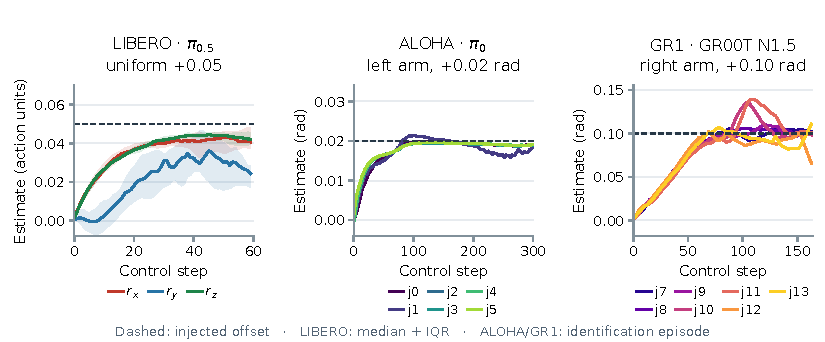
\includegraphics[width=\linewidth]{fig_convergence.pdf}
\caption{\textbf{Historical fault-estimate traces on three robots.}
Left: LIBERO spatial, $\pi_{0.5}$, uniform $+0.05$ command offset and rotation-only
correction; rotation-channel medians and interquartile ranges over 20 episodes for the
first 60 updates. Two medians exceed $0.04$ by the last plotted update; the third is
$0.024$. Middle: ALOHA transfer-cube, $\pi_0$, $+0.02$\,rad on six left-arm joints;
the identification episode ends at $0.0183$--$0.0191$\,rad, then held
(\S\ref{sec:aloha}). Right: GR1, GR00T N1.5, $+0.10$\,rad on seven right-arm joints;
one 164-step identification episode. Its final-50-step average, used for held correction,
is $0.090$--$0.112$\,rad across joints (\S\ref{sec:gr1}). This average does not imply
sustained convergence by step 100. Dashed lines denote the injected offsets.
The panels describe estimation under different protocols, not comparative task success.}
\label{fig:convergence}
\end{figure}

\subsection{Protocol}

\textbf{Paired design.} Except for the unpaired GR1 study (\S\ref{sec:gr1}), compared arms target the same (task, initial state)
episodes and differ only in whether the correction is applied; the policy's own sampling
noise is not pinned across arms, so pairing is on the episode, not on the realised action
sequence. Figure~\ref{fig:convergence}
shows what the corrected arm does inside one episode. We report exact McNemar tests
on the discordant pairs. ``Fixed'' and ``broken'' denote observed outcome differences,
which include policy sampling variability. Historical logs do not certify full physical
state pairing retrospectively; new confirmations verify physical-state and model fingerprints.
\textbf{Controls and uncertainty.} Healthy controls distinguish repair from baseline
competence, but a nonsignificant difference does not establish equivalence or absence of
harm. Three repeated historical cells scored $13/20$, $13/20$, $15/20$; this illustrates
sampling variation, not a general $\pm10$-point error bound. Unless otherwise stated,
historical per-cell $p$-values are unadjusted; the four-suite headline also survives
Bonferroni correction across its four suites. New studies state their comparison families.
\textbf{Calibration.} The original plant and $M$ were identified on
\code{libero\_spatial} healthy rollouts with $\pi_{0.5}$ driving and are used unchanged for
the original LIBERO suites and backbone-transfer experiments; historical ALOHA and GR1
use separate calibrations from eight and six healthy rollouts, respectively.
Original LIBERO calibration overlaps evaluated task/initial
state combinations, so those tables do not establish fully held-out calibration. New
Panda confirmations use disjoint, suite-specific calibration; the latest ALOHA estimator
study uses separately recorded calibration, tuning and confirmation cohorts. These new
protocols do not retroactively repair old provenance.

\subsection{Four suites}
\label{sec:headline}

Uniform $+0.05$ offset on all six action dimensions, rotation-only correction
(\S\ref{sec:channels}), $\pi_{0.5}$-LIBERO.

\begin{center}\small
\begin{tabular}{lrrrrrc}
\toprule
suite & $n$ & frozen & corrected & fixed & broken & exact McNemar \\
\midrule
\code{libero\_spatial} & 20 & 8/20 (40\%) & 18/20 (90\%) & 10 & 0 & $0.0020$ \\
\code{libero\_goal}    & 40 & 15/40 (38\%) & 29/40 (72\%) & 15 & 1 & $0.00052$ \\
\code{libero\_object}  & 20 & 5/20 (25\%) & 16/20 (80\%) & 11 & 0 & $0.00098$ \\
\code{libero\_10}      & 40 & 0/40 (0\%) & 15/40 (38\%) & 15 & 0 & $6.1\times10^{-5}$ \\
\midrule
\textbf{pooled} & 120 & \textbf{28/120 (23\%)} & \textbf{78/120 (65\%)} & \textbf{51} & \textbf{1} & $\mathbf{2.4\times10^{-14}}$ \\
\bottomrule
\end{tabular}
\end{center}

Every suite is individually significant. The long-horizon suite goes from a frozen policy
that never succeeds in forty episodes to fifteen recoveries. The single regression is a
\code{goal} episode the frozen policy itself solves three times in four, with an
ordinary-sized correction. \code{libero\_90}, on which the checkpoint was never fine-tuned,
scores $6/20$ unfaulted and is reported as a competence floor of the policy, not a repair
result.

\subsection{Fault families and severity}
\label{sec:severity}
Figure~\ref{fig:map} and the table give the fault-family by magnitude map
(two cells at $n=40$ in Appendix~\ref{app:map40}; constants ablation in Appendix~\ref{app:abl}).

\begin{figure}[t]
\centering
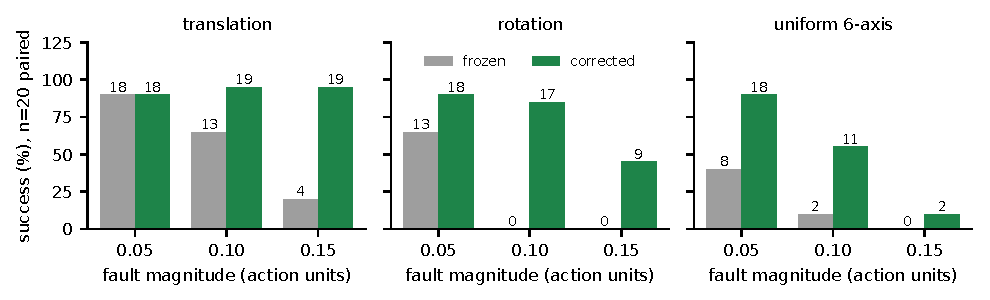
\includegraphics[width=0.92\linewidth]{fig_map.pdf}
\caption{The recoverability map: frozen versus corrected success on LIBERO spatial, $n=20$
paired episodes per cell, correction on the channels each family's separation test
supports (rotation for the rotation and uniform families, translation for translation).
Every regression in the map occurs in a ceiling cell where the frozen policy already
scores 18--19 of 20 (translation $0.05$: one fixed, one broken). Single-family faults
degrade gracefully with magnitude; the
uniform fault collapses at $0.15$ because its uncorrected translation component drives the
arm into contacts and limits (\S\ref{sec:fail}). Exact McNemar $p$-values are in the table
below.}
\label{fig:map}
\end{figure}

\begin{center}\small
\begin{tabular}{lccc}
\toprule
fault (\code{libero\_spatial}, $n=20$) & $0.05$ & $0.10$ & $0.15$ \\
\midrule
translation & 18/20 $\to$ 18/20 (ceiling) & 13/20 $\to$ \textbf{19/20} & 4/20 $\to$ \textbf{19/20} \\
rotation    & 13/20 $\to$ 18/20 & 0/20 $\to$ \textbf{17/20} & 0/20 $\to$ \textbf{9/20} \\
uniform 6-axis & 8/20 $\to$ 18/20 & 2/20 $\to$ 11/20 & 0/20 $\to$ 2/20 \\
\bottomrule
\end{tabular}
\end{center}

No cell outside the ceiling row shows a regression; the translation $0.05$ cell, whose
totals are equal at $18/20$, contains one fixed and one broken episode. Rotation is where
this policy breaks---a rotation fault at
$0.10$ takes it to exactly zero where translation leaves $13/20$---and the correction
recovers $17/20$ from that floor. Single-family faults degrade gracefully with severity; the
uniform fault collapses, and the comparison of the last column isolates why: the rotation
fault and the uniform fault are corrected identically, and adding an \emph{uncorrected}
translation component drops recovery from $45\%$ to $10\%$. This is consistent with a loss
of useful residual information outside the calibrated regime, but does not isolate plant,
estimator and controller contributions. A structured
mixed-sign fault $[0,0,0,+.06,-.06,+.03]$ the law was never tuned on goes $2/12\to10/12$ with
separation matching truth on every axis.

\textbf{Time-varying faults} (amplitude $0.10$): a ramp to full over 60 steps goes
$12/20\to18/20$ ($p=0.031$); a non-zero-mean oscillation on rotation $13/20\to20/20$
($p=0.016$); an intermittent fault $12/20\to19/20$ ($p=0.039$). The estimator tracks the
waveform poorly---$45$--$79\%$ RMS error, not attributable to lag---and it does not matter:
the correction must be roughly right in direction and scale, not a good tracker, which is
why six numbers updated on CPU suffice. (A zero-mean oscillation averages away and does no
damage; that cell proved nothing and is not counted.)

\textbf{Loss of effectiveness} (\S\ref{sec:gain}): at $g=0.30$, $1/20\to17/20$
($p=3.1\times10^{-5}$) with $\hat\beta = (-0.723,-0.699,-0.717)$ against $-0.700$; at
$g=0.20$, $0/20\to17/20$ ($p=1.5\times10^{-5}$). At $g=0.5$ the frozen policy still scores
$15/20$ and the cell is a ceiling. Rotation gain faults are unidentifiable for this policy:
no recorded step clears the excitation gate on $r_x$ or $r_z$ at any threshold, because the
policy does not rotate the wrist. That is a property of the policy's behaviour, not of the
estimator.

\subsection{Baselines}
\label{sec:baselines}

\textbf{Frozen} and a \textbf{static oracle} provide controls. An oracle cancels a known
additive command offset, but is not an empirical upper bound on stochastic task success.
The historical \textbf{raw-error integral} baseline,
$\fhat\leftarrow\fhat+k_i(y_t-a_t)$, was swept over five gains. On the $0.15$ translation
cell its best setting reaches $7/20$ against $19/20$ for calibrated adaptation. This
comparison changes the residual model as well as the update, so it cannot isolate the
adaptive law's contribution or attribute all benefit to $M$ alone.

A later matched-residual pilot keeps the calibrated FIR and sensitivity shared:
original proposed $19/20$, disturbance observer (DOB) $17/20$, recursive least squares
(RLS) $17/20$, Kalman $18/20$, calibrated integral $15/20$, and oracle $20/20$.
All estimated arms retain projection; the DOB removes the legacy deadzone and
normalisation. These small samples support repair through several estimators, but establish
neither equivalence nor a special advantage of the proposed update. The larger, separately
calibrated ALOHA comparison below addresses tuning on its own benchmark.

\subsection{Faults below the controller}
\label{sec:joint}

Command-interface offsets and physical joint faults enter at different levels. An additive
torque is matched relative to joint-torque inputs; whether it can be compensated through
a restricted Cartesian command interface requires a separate response analysis.
Configuration dependence alone does not establish unmatched uncertainty.

The historical Panda study concentrated on elbow joint 3, with continuously updated,
translation-only correction. Its stored outcomes are retained here for provenance:
\begin{center}\small
\begin{tabular}{lrrrrrc}
\toprule
historical elbow fault & $n$ & off & corrected & fixed & broken & McNemar \\
\midrule
torque bias 5\,N\,m & 40 & 20/40 & 32/40 & 15 & 3 & $0.0075$ \\
friction $+10$ & 20 & 11/20 & 14/20 & 6 & 3 & $0.51$ \\
friction $+20$ & 20 & 0/20 & 8/20 & 8 & 0 & $0.0078$ \\
lock $\pm0.05$\,rad & 20 & 0/20 & 0/20 & 0 & 0 & --- \\
\bottomrule
\end{tabular}
\end{center}
The old runner did not restore model faults on every episode exit, so friction and joint
limits could persist across cached resets; those logs lack the model-state snapshots
needed to certify fault severity. Their efficacy claims require reruns under the repaired
lifecycle. A failure with this lock intervention does not prove that task recovery through
other joints is impossible.

The historical seven-joint torque map totals $103/140$ with correction off and on, with
20 observed rescues and 20 regressions. Joint 5 falls from $12/20$ to $3/20$
(Bonferroni-7 $p=0.02734$); joint 6 improves numerically from $7/20$ to $11/20$.
The correction was continuously updated, so a constant-correction explanation is incorrect.
These historical outcomes motivated new full-state-verified experiments.

\textbf{Independent all-joint confirmations.} We completed 1,440 Panda rollouts on
LIBERO Spatial, Object and Goal: seven $+5$\,N\,m joint faults plus healthy, 20 scenarios
per cell, and off/legacy translation/weighted full correction. Fresh calibration is
\emph{suite-specific}: FIR uses all ten tasks at initial state 26; sensitivity probes use
task 0 at initial state 25; confirmation uses all ten tasks at states 35/36. The weighted
allocator solves a bounded, covariance-weighted ridge problem over permitted inputs.
It changes both support and regularisation, so this comparison does not isolate either.
The registered joint-5 comparison improves from legacy $15/60$ to weighted $41/60$
(29 rescues, 3 regressions, $p=2.556\times10^{-6}$). Against off, $36/60$ versus $41/60$
is descriptive. Weighted correction harms Object joint 3 relative to legacy
($16/20\to2/20$, Bonferroni-24 $p=0.01245$; off $8/20$). Legacy itself harms healthy
Goal ($19/20\to3/20$, adjusted $p=0.00073$). Thus neither implementation supports
uniform repair or a no-harm claim.

A separate 780-rollout ALOHA transfer test covers all twelve arm joints plus healthy,
20 seeds per cell and three arms. The weighted allocator uses the historical ALOHA
sensitivity; complete original calibration-seed provenance is unavailable. Faulted totals
are off $60/240$, legacy $70/240$, weighted $66/240$; healthy is $11/20$, $8/20$, $6/20$.
No cell resolves after its declared Bonferroni-13 correction, which establishes neither
transfer benefit nor equivalence. This is weighted allocation, not the composite observer:
the twelve-joint position reference failed qualification. Full settings and counts are in
Appendix~\ref{app:joint}.

\textbf{Mechanism remains partial.} Repeated local physical probes distinguish model fit
from actual compensation. After observer initialisation, legacy translation worsens the
scaled local physical error in 150/168 probes; weighted full does so in 92/168, despite
passing every fitted-objective check. One weighted solution reduces the model objective
to $10.5\%$ of zero correction while increasing physical error in the same covariance
metric $2.69$-fold. On ALOHA, privileged command shifts of $-\tau/k_p$ cancel all 144 tested
local torque responses to numerical precision. These interventions establish local command
authority and model-response mismatch; they do not identify the cause of each task failure
or guarantee task recovery. The weighted variant remains experimental.

\subsection{Two further backbones, unchanged calibration}
\label{sec:oft}

OpenVLA-OFT (7B, autoregressive backbone with an L1 action head) and NVIDIA GR00T N1.7
(3B, Cosmos VLM with a flow-matching DiT head, the official LIBERO finetune) are each
served behind the same interface; every script, the plant and $M$ are the $\pi_{0.5}$ ones.

\begin{center}\small
\begin{tabular}{lrrrrc}
\toprule
cell (\code{libero\_spatial}) & frozen & corrected & fixed & broken & McNemar \\
\midrule
healthy control & 20/20 & 19/20 & 0 & 1 & 1.0 \\
rotation $0.10$ & 0/20 & \textbf{11/20} & 11 & 0 & $9.8\times10^{-4}$ \\
translation $0.15$ & 0/20 & \textbf{14/20} & 14 & 0 & $1.2\times10^{-4}$ \\
gain $0.20$ & 0/20 & \textbf{17/20} & 17 & 0 & $1.5\times10^{-5}$ \\
\bottomrule
\end{tabular}
\end{center}

Nothing in the method was $\pi_{0.5}$-specific. OFT is more fragile (frozen $0/20$ on all
three faults), recovers less on rotation ($55\%$ vs $85\%$; its $r_y$ fault is only $23\%$
identified where $\pi_{0.5}$ reached $87$--$100\%$), and the healthy control lost one episode
to the law itself: a sustained phantom at four to ten times the usual size, which a
confidence gate evaluated offline does not remove without delaying genuine repair by one to
two seconds (\S\ref{sec:fail}). The three headline cells also replicate on
\code{libero\_object} with the same calibration ($0/20\to10/20$, $0/20\to15/20$,
$0/20\to19/20$).

GR00T N1.7 is a third developer and a third architecture. Its healthy control is a null on
totals ($18/20$ both arms, one fixed and one broken, rotation phantom below $0.005$). With no retuning: rotation $0.10$,
$0/20\to\mathbf{14/20}$ (14 fixed, 0 broken, $p=1.2\times10^{-4}$); translation $0.15$,
$2/20\to\mathbf{15/20}$ (13/0, $p=2.4\times10^{-4}$); gain $0.20$ under the multiplicative
law, $0/20\to\mathbf{19/20}$ (19/0, $p=3.8\times10^{-6}$, $\hat\beta$ within $2\%$ of the
true $-0.80$). Three families, 46 repaired, none broken. The under-identified $r_y$ is the same channel that lags on the other two
backbones: it is a property of the plant and $M$, not of the policy. Across the three
backbones on this cell, 42 of 60 paired episodes are repaired and none is broken.

That last figure needs its denominator stated, and so does every regression count in this
paper. A regression can only occur in an episode the frozen policy was already winning.
Across the full $3\times3$ transfer table, seven of the nine cells have a frozen policy at
exactly $0/20$: of $180$ paired episodes, only $\mathbf{6}$ were successes that the
correction could have broken. \emph{None broken in $180$ episodes} is therefore none broken
in six opportunities, an exact $95\%$ upper bound of $39.3\%$ on the regression rate, not
the $1.7\%$ that a denominator of $180$ would suggest. The stronger reading is not available
from these cells. We report both denominators throughout; the second is the one that answers
\emph{if I switch this on, how often does it break something that was working}.

\subsection{A second manipulator, in joint space}
\label{sec:aloha}

Bimanual ALOHA in \code{gym\_aloha} driven by $\pi_0$: fourteen absolute joint targets at
50\,Hz, transfer-cube, 300-step episodes, healthy success $25\%$. The plant is identified on
\emph{position} from eight healthy rollouts (in-sample $R^2 = 0.989$--$1.000$ on the arm joints; right gripper $0.768$),
$M\approx I$. A $+0.05$\,rad offset on the six left-arm joints displaces the gripper by
$5.3$\,cm; the frozen policy scores $0/20$ at every severity tested.

\textbf{Identification transfers.} Separation against the healthy control: $85$--$91\%$ of
the fault at $0.05$\,rad, $94$--$106\%$ at $0.02$\,rad, leakage $\le0.007$\,rad onto
uncorrected joints. \textbf{Repair does not, at first.} With continuous adaptation the task
returns $0/20$ at every severity, warm-started or cold, with or without an early-history
defect we found and fixed. The historical comparison is:

\begin{center}\small
\begin{tabular}{lccc}
\toprule
correction & variation & mean residual & success \\
\midrule
none (frozen) & --- & 2.12\,cm & 0/20 \\
adaptive, updating throughout & 0.43\,cm & 0.17\,cm & 0/20 \\
$0.019$\,rad ($95\%$) applied frozen & 0 & 0.11\,cm & \textbf{5/20} \\
Identify, then hold ($n=40$) & 0 after episode 0 & 0.12\,cm & \textbf{15/40} \\
Healthy, law off ($n=40$) & --- & --- & 17/40 \\
\bottomrule
\end{tabular}
\end{center}

The fault is $+0.02$\,rad and $n=20$ unless otherwise stated. Identify-then-hold versus
frozen has $p=6.1\times10^{-5}$ with no observed regressions. In the historical static sweep, a $90\%$ correction restores no successes while a $100\%$
correction reaches the observed healthy rate. These data suggest sensitivity to correction
accuracy and timing, but do not isolate variation as the cause of continuous adaptation's
failure. The identify-then-hold total $15/40$ includes one failed identification episode
and 39 episodes using its held estimate ($0.019$--$0.020$\,rad); only those latter episodes
have zero within-episode correction variation. Its difference from healthy $17/40$ remains
unresolved ($p=0.75$), without establishing equivalence. The historical healthy comparison
$14/40$ versus $17/40$ has five rescues and eight regressions ($p=0.58$).

These results use the original all-channel normaliser and calibration. They are not
results for the corrected-channel setting or the fresh calibration used in
\S\ref{sec:composite}. The later tuned continuous observer succeeds in some offset episodes,
so the historical zero-success result is not a general boundary of continuous adaptation.

\subsection{A humanoid}
\label{sec:gr1}
Fourier GR1 upper body (two 7-joint arms, two 6-joint hands, a waist; 29 absolute joint
targets at 20\,Hz) in RoboCasa, driven zero-shot by GR00T N1.5, for which GR1 is a
pretrained embodiment. Plant from six healthy
episodes ($R^2\ge0.998$ on the arm), $M$ by direct step response ($0.99\,I$ on the arm
block; the replay probe of \S\ref{sec:aloha} is contaminated on an arm in contact),
constants from the measured residual. A $+0.10$\,rad offset on the working arm zeros the
policy on both tasks. The simulator's scene generator is reseeded per episode so both arms
see identical scenes. The estimate is the median over three episodes of the reach-window
(steps 50--200) estimate: an episode's end reads a contact standoff, $0.2$\,rad wrong on a
wrist on two of three draws.

\begin{center}\small
\begin{tabular}{lrrrrrcc}
\toprule
task, $n=30$ paired & healthy & frozen & corrected & fixed & broken & McNemar & vs healthy \\
\midrule
plate-to-plate & 22/30 & 1/30 & \textbf{19/30} & 18 & 0 & $7.6\times10^{-6}$ & $p=0.55$ \\
tray-to-plate & 17/30 & 1/30 & \textbf{13/30} & 12 & 0 & $4.9\times10^{-4}$ & $p=0.45$ \\
\bottomrule
\end{tabular}
\end{center}

Held vectors are $93$--$104\%$ and $73$--$126\%$ of the fault per joint; on a healthy arm
the law changes nothing ($19/30$ vs $18/30$; $16/30$ vs $15/30$); continuous adaptation
reaches $8/30$, a third of the ceiling. Appendix~\ref{app:gr1map} maps three magnitudes.

\subsection{A second simulator: WidowX in SimplerEnv}

The earlier GR1 cohorts (runs before the scene generator was reseeded, unpaired, Fisher
tests: held $21/30$ against pooled frozen $4/90$ and healthy $64/90$) are kept in the record
and in the audit's merge notes; the paired cells above supersede them as the GR1 evidence.

\subsection{A second simulator: WidowX in SimplerEnv}
\label{sec:widowx}
SimplerEnv \citep{li2024simpler} runs in SAPIEN; GR00T N1.7's Bridge finetune drives a
WidowX on \emph{put the spoon on the towel} with Cartesian pose increments on an
accumulating target. Plant from ten healthy episodes, $M$ the plant's DC gain (the held-pose
probe is wrong on $z$ here), constants from the residual. A $+0.005$ offset on $x,y,z$,
$2.5\times$ the residual, zeros the policy. The estimate lands on the fault (median $0.0050$,
$0.0051$, $0.0049$), but the drift during its 27-step transient stays in the target:
online adaptation reaches $6/20$ against a healthy $13/20$ ($6$ fixed, $0$ broken), and
$12/20$ ($12$ fixed, $0$ broken) with the gain raised to halve the transient. Identify over
three episodes and hold: on the next $20$ paired episodes healthy $14/20$, frozen $0/20$,
corrected $\mathbf{14/20}$ ($14$ fixed, $0$ broken, $p=1.2\times10^{-4}$; vs healthy
unresolved, $p=1.0$), the ALOHA and GR1 scheme, same reason.

\subsection{Composite adaptation and independent estimator tuning}
\label{sec:composite}

\textbf{Variant.} A fitted healthy position model gives
$q^{\rm ref}_{t+1}=Aq^{\rm ref}_t+B a_t+c$ from the raw policy command, with no velocity
tracking term. The FIR residual instead uses the corrected, pre-fault command. Let
$e^q_{t+1}=q_{t+1}[J]-q^{\rm ref}_{t+1}$, let $D=B\operatorname{diag}(m)$ include the correction
mask. Here $J=\{0,\ldots,5\}$, $q^{\rm ref}_0=q_0[J]$, and $L\succ0$ is the fitted
model's contraction metric. The implemented discrete
composite update is
\begin{equation}\label{eq:composite}
\hat\theta_{t+1}=\Pi_{[-\kappa,\kappa]}\!\left[
 a_\lambda\hat\theta_t+K_t(z_{t+1}-M a_\lambda\hat\theta_t)
 +\Delta t\,\eta P^+_t D^\top L e^q_{t+1}\right],
\end{equation}
where $a_\lambda=\exp(-\lambda\Delta t)$, $z=r-Mb_f$, $K_t$ is the Kalman gain and
$P^+_t$ its Joseph-form posterior covariance, carried forward as $P_{t+1}=P^+_t$. Specifically,
$K_t=P^-_tM^\top(MP^-_tM^\top+R)^{-1}$. The tuned ALOHA implementation uses
$b_f=0$ (the FIR intercept remains). The prior is
$P^-_t=a_\lambda^2P_t+Q_c(1-a_\lambda^2)/(2\lambda)$, with the continuous limit
$P_t+\Delta t Q_c$ at $\lambda=0$. Setting $\eta=0$ gives the same damped Kalman recursion;
setting both $\eta$ and $\lambda$ to zero gives an undamped Kalman filter with identical
$Q_c,R,P_0$ and clipping, not the differently tuned selected Kalman configuration. The action uses the
old estimate, then the new position updates the estimate for the next action. No injected
fault value enters the estimated arms. This is an action-interface variant inspired by
composite adaptation, not a reproduction of Neural-Fly's force controller or its guarantee.

\textbf{Qualification and split.} Fresh ALOHA data use 20 healthy fitting episodes
(seeds 3100--3119) and ten qualification episodes (3120--3129). Sensitivity probes reuse
three fitting donors with exact physical-state resets. The left-six position model passes
the declared $0.005$-rad maximum per-coordinate one-step and rollout-RMSE gates
(maximum rollout RMSE $0.00332$); its fitted-metric
contraction factor is $0.895$. The full twelve-arm-joint model fails prediction qualification.
Neither a contracting fitted model nor the local augmented-system checks prove contraction
of the complete healthy VLA--robot loop.

The bank contains 24 original-law, 12 DOB, 24 RLS, 24 Kalman, 72 composite and 12 calibrated
integral recipes, plus off and oracle. Seven composite recipes fail the fixed local
stability screen. All 163 eligible arms enter a 2,608-rollout search; a separate
896-rollout validation selects one candidate per estimated family; 1,920 confirmation
rollouts evaluate those six and two controls on 30 untouched seeds. In total, 5,424
evaluation rollouts were completed. The larger composite search pool and the finite bank
are disclosed; no parameter is selected from confirmation outcomes.

\textbf{Confirmation.} All runs use ALOHA Transfer Cube, left-six correction, 50\,Hz,
300-step episodes and ten-action chunks. Conditions are healthy, $+0.02$\,rad command
offset on those six joints, and individual left-joint torque faults
$[16,32,16,0.2,1,0.4]$\,N\,m. With seven fault rates $p_j$ and healthy rate $p_h$, the
predeclared score is $S=\tfrac12p_h+\tfrac1{14}\sum_{j=1}^7p_j$, not the unweighted
success fraction over 240 episodes.
\begin{center}\small
\begin{tabular}{lrrr}
\toprule
selected method/control & healthy & faulted & balanced score \\
\midrule
Original proposed & 16/30 & 98/210 & 50.00\% \\
RLS & 17/30 & 63/210 & 43.33\% \\
DOB & 14/30 & 79/210 & 42.14\% \\
Kalman & 12/30 & 71/210 & 36.90\% \\
Composite & 12/30 & 67/210 & 35.95\% \\
Calibrated integral & 11/30 & 57/210 & 31.90\% \\
\midrule
Off & 15/30 & 48/210 & 36.43\% \\
Oracle (unranked) & 13/30 & 103/210 & 46.19\% \\
\bottomrule
\end{tabular}
\end{center}
Composite minus Kalman is $-0.95$ percentage points (whole-seed bootstrap $95\%$ interval
$[-9.52,7.62]$; exact whole-seed sign-flip $p=0.86261$). Seed clustering preserves repeated
scenarios across conditions. The four secondary overall Kalman comparisons do not survive
Holm correction; this table is a numerical ordering, not an established ranking.
In the offset cell, DOB scores $9/30$ versus Kalman $0/30$ (Bonferroni-8 $p=0.03125$
within that contrast's eight-condition family). No composite--Kalman cell survives its
Bonferroni-8 correction. The oracle is exact for offsets and nominal $\tau/k_p$ for torque,
with independent policy sampling; it is not a task-success upper bound.

\textbf{Diagnosis.} Across all confirmation conditions, composite lowers late-window
position-reference RMS error, yet more than $99.39\%$ of the squared tracking increment
on corrected coordinates lies on joint 1. In the exact-offset cell, late parameter RMS error increases from Kalman's
$0.00511$ to composite's $0.00576$\,rad while reference RMS falls from $0.00950$ to
$0.00747$\,rad. No sign, timing or covariance-recursion defect was identified; better
reference tracking does not guarantee better task success. Only one composite episode
has active-coordinate clipping (12 late updates), so broad clipping does not explain the
ranking. The selected configurations differ in bandwidth, damping and clipping; isolating
the extra tracking term requires a matched-parameter ablation on fresh scenarios.
Full selected settings are in Appendix~\ref{app:tuning}.

\subsection{Hardware}
\label{sec:hardware}
The X2 humanoid protocol (a real actuator-authority fault in 134 logged rollouts, invisible in position, recoverable in effort) is in Appendix~\ref{app:hw}; paired repair on the robot remains pending.

\section{Additional empirical diagnostics}
\label{sec:fail}

\textbf{Invisible faults.} Neither a proprioceptive bias nor a wrist-camera misalignment
reaches the residual (separation $0.004$ against $0.049$ for an action fault): the method
sees the action interface and nothing upstream of it. The proprioceptive bias does not
damage the policy either --- it scores $15/15$ and $12/12$ frozen --- which follows from
Appendix~\ref{app:adapterstate}: the tested checkpoint ignores that state input, so the method's blind
spot and the policy's coincide. The camera perturbation is an image shift (\code{np.roll}),
not a physical extrinsic change, and damages the policy ($6/12$) without being observable.

\textbf{A policy that cannot do the task.} \code{libero\_90} fails 14 of 20 sampled tasks
unfaulted. Correcting the fault restores nothing because nothing was lost to it.

\textbf{Harm on healthy and faulted robots.} The historical OFT regression coincides with a
sustained phantom estimate. The new studies add much larger counterexamples: legacy
translation harms healthy LIBERO Goal, weighted full harms Object joint 3 versus legacy,
and the ALOHA healthy weighted success count decreases (\S\ref{sec:joint}). A gate evaluated
offline or a nonsignificant test cannot establish that deployment is harmless.

\textbf{Mechanistic claims revised.} Healthy action statistics alone did not predict every
identifiable channel: translation identifies a single-family fault at $79\%$--$106\%$.
Measured single-axis sensitivity changes by at most $14\%$ across the tested probes, while
multi-axis superposition fails; this does not prove global linearity or identify a specific
contact mechanism. Translation correction can help under its own fault family. Conversely,
configuration dependence does not explain the joint-5 harm by itself, and continuous
corrections cannot be described as a constant estimate becoming stale. These observations
motivate controlled interventions rather than a closed causal explanation.


\section{Ablation of the law's constants and the calibration size}
\label{app:abl}
Headline cell ($\pi_{0.5}$, \code{libero\_spatial}, uniform $+0.05$, rotation-only
correction), $n=20$ paired per row, one constant changed per row from the reference
($\gamma=0.08$, $\rho=0.15$, deadzone $0.008$, plant fitted on three healthy episodes,
285 steps). Last column: rotation estimate at episode end (last-50-step mean) against a
true $0.05$ on each axis.

\begin{center}\small
\resizebox{\linewidth}{!}{
\begin{tabular}{lrrrrcl}
\toprule
setting & frozen & corrected & fixed & broken & McNemar & $\hat f_{rx},\hat f_{ry},\hat f_{rz}$ \\
\midrule
reference & 8/20 & \textbf{18/20} & 10 & 0 & $0.0020$ & 0.044, 0.020, 0.044 \\
$\gamma=0.02$ ($\tfrac14\times$) & 8/20 & 17/20 & 9 & 0 & $0.0039$ & 0.036, 0.016, 0.036 \\
$\gamma=0.32$ ($4\times$) & 7/20 & 18/20 & 11 & 0 & $0.00098$ & 0.044, 0.019, 0.044 \\
$\rho=0.05$ ($\tfrac13\times$) & 11/20 & 14/20 & 5 & \textbf{2} & $0.45$ & 0.027, 0.011, 0.027 \\
$\rho=0.50$ ($3\tfrac13\times$) & 8/20 & \textbf{20/20} & 12 & 0 & $0.00049$ & 0.048, 0.022, 0.049 \\
deadzone $0$ & 8/20 & 19/20 & 11 & 0 & $0.00098$ & 0.044, 0.018, 0.044 \\
deadzone $0.03$ ($\approx$ residual scale) & 8/20 & 17/20 & 9 & 0 & $0.0039$ & 0.031, 0.016, 0.032 \\
plant from 1 healthy episode (75 steps) & 10/20 & 17/20 & 8 & 1 & $0.039$ & 0.027, 0.008, 0.044 \\
plant from 2 healthy episodes & 8/20 & 17/20 & 10 & 1 & $0.012$ & 0.045, 0.021, 0.043 \\
\bottomrule
\end{tabular}}

\end{center}

Within this historical cell, the three tested gains give similar success counts; the
experiment does not establish parameter insensitivity across faults or robots. The smaller
normalisation radius has two regressions and a weaker observed benefit, consistent with
its attenuated target. One healthy episode yields $17/20$ despite under-identification on
one rotation axis. These are cell-specific ablations with unadjusted tests, not evidence
that this calibration size or parameter range is sufficient in general.

\section{Hardware protocol on the X2 humanoid}
\label{app:hw}
On logs from an X2 humanoid running a learned box-pickup policy, a real actuator-authority
fault (stiffness, damping and feedforward scaled together, $0.1$--$1.3$ across 134
rollouts) is invisible in joint position and recoverable in effort ($r=+0.84$); the plant
is run-varying on load-bearing joints, so calibration must be within-run and in motion; the
detectability floor is $0.5$--$1.3^\circ$ of joint offset. Paired repair on
the robot remains pending.

\section{Humanoid recoverability map}
\label{app:gr1map}
Plate-to-plate, right-arm offset at three magnitudes, paired on identical scenes, identify
over three episodes then hold (\S\ref{sec:gr1}), $n=30$ per arm:

\begin{center}\small
\begin{tabular}{lrrrrrcl}
\toprule
offset & healthy & frozen & corrected & fixed & broken & McNemar & held estimate \\
\midrule
$0.05$\,rad & 19/30 & 7/30 & \textbf{24/30} & 17 & 0 & $1.5\times10^{-5}$ & $90$--$108\%$ \\
$0.10$\,rad & 22/30 & 1/30 & \textbf{19/30} & 18 & 0 & $7.6\times10^{-6}$ & $93$--$104\%$ \\
$0.20$\,rad & 25/30 & 0/30 & \textbf{21/30} & 21 & 0 & $9.5\times10^{-7}$ & $94$--$99\%$ \\
\bottomrule
\end{tabular}
\end{center}

Every cell is at its healthy rate ($p=0.18$, $0.55$, $0.29$ against the healthy arm) with no
regression in 90 paired episodes; at $0.20$\,rad ($11.5^\circ$ on every joint of the working
arm) the frozen policy never succeeds. The identification stays within $10\%$ across a
fourfold range of magnitude, with no sign of the superposition boundary the Panda shows at
its largest uniform fault (\S\ref{sec:severity}).

\paragraph{Time-varying faults on the humanoid.} Same cell, $n=20$ paired, amplitude
$0.10$\,rad. A ramp to full over 60 steps is constant thereafter, and the held estimate
serves it: $1/20\to11/20$ (10 fixed, 0 broken, $p=0.002$; healthy $13/20$, $p=0.73$).
Continuous adaptation repairs the ramp significantly but below healthy ($9/20$, $p=0.021$
against frozen, $p=0.039$ against healthy $16/20$), lagging the rise by about 30 steps and
then continuing to move. The two profiles that never settle are the boundary: a slow
non-zero-mean oscillation reaches $6/20$ and an intermittent fault $4/20$, neither
significant against frozen at $n=20$. On the Panda the same profiles were repaired
(\S\ref{sec:severity}) because a Cartesian reach tolerates a correction that is briefly
wrong; a dexterous-hand grasp does not, which is the hypothesis in \S\ref{hyp:repair} on the
axis it names: a fault that keeps moving cannot be given a stationary correction.

\section{Recoverability-map cells at \texorpdfstring{$n=40$}{n=40}}
\label{app:map40}
Two borderline historical cells of \S\ref{sec:severity} were selectively expanded to
$n=40$ (same configuration, initial states 45--48). Rotation $0.05$ originally scored
$13/20\to18/20$, five rescues and no regressions ($p=0.0625$). At $n=40$, rotation
$0.05$: $27/40\to39/40$, 12 fixed, 0 broken, $p=4.9\times10^{-4}$. Translation $0.10$:
$30/40\to38/40$, 9 fixed, 1 broken, $p=0.021$. These unadjusted historical follow-ups
were not a preregistered confirmation family; uniform $0.15$ remains unresolved.

\section{All-joint physical-fault confirmation details}
\label{app:joint}
Panda entries are off / legacy translation / weighted full successes out of 20.
Each fault is $+5$\,N\,m; healthy is zero. Both estimated arms use $\gamma=0.08$ and
clipping $0.30$; weighted allocation uses prior standard deviation $0.1$ in command units.
Spatial/Object/Goal use 220/280/300-step limits and five-action chunks.
\begin{center}\small
\begin{tabular}{lccc}
\toprule
condition & Spatial & Object & Goal \\
\midrule
Healthy & 20/19/20 & 20/18/20 & 19/3/19 \\
Joint 0 & 19/20/20 & 20/5/19 & 20/3/20 \\
Joint 1 & 19/19/19 & 19/17/16 & 16/5/17 \\
Joint 2 & 18/19/19 & 15/1/19 & 16/5/16 \\
Joint 3 & 13/15/19 & 8/16/2 & 7/4/11 \\
Joint 4 & 15/16/20 & 12/13/16 & 10/5/19 \\
Joint 5 & 14/6/17 & 11/5/9 & 11/4/15 \\
Joint 6 & 8/11/20 & 6/0/15 & 8/2/10 \\
\bottomrule
\end{tabular}
\end{center}
The primary pools only the 60 distinct joint-5 scenarios. Per-cell tests retain three
separate 24-comparison families (one per method contrast). Repeated scenarios across
fault cells are not pooled as independent observations in a significance test.

ALOHA entries use 20 seeds (3000--3019), 300-step limits, $\gamma=0.08$, clipping $0.08$
and weighted prior standard deviation $0.1$ in ALOHA command units. Each arm uses torques
$[16,32,16,0.2,1,0.4]$\,N\,m, equal to nominal $k_p\times0.02$\,rad.
Physical joints 0--11 map to command coordinates 0--5 and 7--12, excluding grippers.
\begin{center}\small
\begin{tabular}{lrrr}
\toprule
condition & off & legacy all-channel norm & weighted \\
\midrule
Healthy & 11 & 8 & 6 \\
Left 0 & 0 & 0 & 0 \\
Left 1 & 8 & 7 & 6 \\
Left 2 & 11 & 7 & 8 \\
Left 3 & 1 & 6 & 6 \\
Left 4 & 4 & 7 & 7 \\
Left 5 & 7 & 6 & 6 \\
Right 0 & 0 & 4 & 5 \\
Right 1 & 6 & 6 & 6 \\
Right 2 & 3 & 9 & 7 \\
Right 3 & 8 & 8 & 4 \\
Right 4 & 7 & 5 & 5 \\
Right 5 & 5 & 5 & 6 \\
\bottomrule
\end{tabular}
\end{center}
Three method contrasts each retain 13 comparisons. These settings and historical
calibration differ from the fresh left-six estimator tuning study below.

\section{Selected estimator settings and confirmation cells}
\label{app:tuning}
The six selected recipes are frozen before confirmation. With healthy residual covariance
$R$, define $C=M^{-1}RM^{-\top}$. The matched recipe is
$Q_{\rm step}=\gamma^2C/(1-\gamma)$ and $Q_c=Q_{\rm step}/\Delta t$; damped propagation
uses the interval in \eqref{eq:composite}. Covariance scale multipliers are one.
\begin{center}\small
\begin{tabular}{lp{0.70\linewidth}}
\toprule
family & selected settings \\
\midrule
Original & $\gamma=.5$, clip $.04$, deadzone $.002$, norm radius $.4$, corrected-channel norm \\
DOB & $\gamma=.5$, clip $.08$ \\
RLS & forgetting $1$, initial covariance $.1I$, clip $.08$ \\
Integral & gain $.005$ per update, clip $.08$ \\
Kalman & matched $Q$, $\gamma=.08$, $P_0=C$, damping $0$, clip $.16$ \\
Composite & matched $Q$, $\gamma=.2$, $P_0=C$, damping $.5$/s, clip $.08$, active tracking strength $.02$ \\
\bottomrule
\end{tabular}
\end{center}
The active strength sets
$\eta=.02/\|[\Delta t P_\infty D^\top L D]_{J,J}\|_2$, where $P_\infty$ is the posterior
steady covariance under the candidate's damping and noise. Thus $.02$ is not the
per-second coefficient $\eta$ itself.
The selected full-precision recipe has $\eta=3017861.266508692$ in the stated coordinates.
The reference is driven by all fourteen raw commands while tracking the six left joints.
Calibrated sensitivity has full rank 14 and condition number $7.0813$.

Search uses seeds 3200--3203 and healthy/offset/joints 1 and 3. Validation uses 3300--3307
on all eight conditions; confirmation uses 3400--3429. Search selects two candidates per
family, validation selects one, and confirmation never changes parameters. The bank includes
24 Kalman and 72 nonzero-tracking composite recipes, with zero-tracking Kalman recipes reused
as controls. It explores bandwidth, covariance initialization and noise form, damping and
clipping; other families also vary their relevant gains, priors, forgetting and norm settings.
A calibrated $Q=0$ static filter needs a different information-growth qualification and is
outside this bank. Parameters are selected within this finite search, not globally optimal.

\begin{center}\small
\begin{tabular}{lrrrrrrrr}
\toprule
method & healthy & offset & J0 & J1 & J2 & J3 & J4 & J5 \\
\midrule
Original & 16 & 7 & 11 & 16 & 15 & 16 & 14 & 19 \\
RLS & 17 & 0 & 0 & 15 & 11 & 10 & 15 & 12 \\
DOB & 14 & 9 & 11 & 14 & 12 & 10 & 12 & 11 \\
Kalman & 12 & 0 & 2 & 17 & 13 & 12 & 16 & 11 \\
Composite & 12 & 2 & 2 & 10 & 12 & 12 & 16 & 13 \\
Integral & 11 & 0 & 0 & 13 & 15 & 7 & 13 & 9 \\
Off & 15 & 0 & 0 & 16 & 10 & 2 & 12 & 8 \\
Oracle & 13 & 13 & 13 & 16 & 14 & 17 & 14 & 16 \\
\bottomrule
\end{tabular}
\end{center}
Each entry is success out of 30. Analysis keeps all eight conditions clustered by seed.
The primary test is exact under whole-seed exchangeability/sign symmetry, not an arbitrary
zero-mean null. It evaluates all $2^{30}$ sign assignments by dynamic programming;
bootstrap intervals use 50,000 whole-seed resamples with analysis seed 20260908 and are
approximate, unadjusted intervals. Four secondary overall contrasts use Holm correction;
per-cell comparisons use five distinct eight-condition families, not one global family
of forty. An independent extraction reproduces all 1,920 outcomes, tests and intervals
from 48 source-verified confirmation archives.



\end{document}
